\documentclass[10pt, nonatbib, nocopyrightspace, reprint]{sigplanconf}

\usepackage{float}
\usepackage[backref=section, linkbordercolor={1 1 1}, urlbordercolor={1 1 1}, citebordercolor={1 1 1}, pdftex,
            pdfauthor={Helium Systems Inc},
            pdftitle={Helium},
            pdfsubject={A Decentralized Wireless Network},
            pdfkeywords={helium, IoT, DWN, wireless},
            pdfproducer={Latex with hyperref},
            pdfcreator={pdflatex}]{hyperref}
\usepackage{microtype}
\usepackage{placeins}
\usepackage{color}
\usepackage{cite}
\usepackage{graphicx}
\usepackage{parskip}
\usepackage{booktabs}
\usepackage{float}
\usepackage{tabularx}
\usepackage{pgfplots}
\usepackage{amsmath}
\usepackage{titlesec}
\usepackage[local]{gitinfo2}
\renewcommand{\gitMark}{Release \gitFirstTagDescribe{} (\gitAuthorDate)}

\graphicspath{ {images/} }

\newcommand{\todo}[1]{}
\renewcommand{\todo}[1]{{\color{red} TODO:\ {#1}}}

\renewcommand{\sectionautorefname}{Section}
\renewcommand{\subsectionautorefname}{Section}
\renewcommand{\subsubsectionautorefname}{Section}
\newcommand{\secref}[1]{[\autoref{#1}]}

\renewcommand{\figureautorefname}{Figure}
\newcommand{\figref}[1]{[\autoref{#1}]}

\renewcommand{\equationautorefname}{Equation}
\renewcommand{\eqref}[1]{[\autoref{#1}]}



\pgfplotsset{compat=newest}

\begin{document}

\special{papersize=8.5in,11in}
\setlength{\pdfpageheight}{\paperheight}
\setlength{\pdfpagewidth}{\paperwidth}

\title{Helium}
\subtitle{A Peer-to-Peer Wireless Network}
\authorinfo{Amir Haleem\and Andrew Allen \and Andrew Thompson \and Marc Nijdam \and Rahul Garg}{Helium Systems, Inc.}{\gitMark}

\maketitle

\begin{abstract}
The Internet of Things is an \textdollar800 billion industry, with over 8.4 billion connected devices online, and spending predicted to reach nearly \textdollar1.4 trillion by 2021~\cite{idc}. Most of these devices need to connect to the Internet to function. However, current solutions such as cellular, WiFi, and Bluetooth are suboptimal: they are too expensive, too power hungry, or too limited in range.

The Helium network is a \emph{peer-to-peer wireless network} that enables devices anywhere in the world to wirelessly connect to the Internet without the need for power-hungry hardware or expensive cellular plans. Powering the Helium network is a blockchain with a native protocol token and a dedicated bandwidth token, incentivizing a two-sided marketplace between coverage providers and coverage consumers. With the introduction of a blockchain, we inject decentralization into an industry currently controlled by monopolies. The result is that wireless network coverage becomes a commodity, fueled by competition, available anywhere in the world, at a fraction of current costs.

Our secure and open-source primitives enable developers to build low-power, Internet-connected devices quickly and cost-effectively. The Helium network has a wide variety of applications across industries and is the first peer-to-peer wireless network of its kind.
\end{abstract}

\section{Introduction}

The world is becoming decentralized. A multitude of platforms, technologies, and services are moving from centralized proprietary systems to decentralized, open ones. Peer-to-peer networks such as Napster (created by one of our founders Shawn Fanning) \cite{napster} and BitTorrent paved the way for blockchain networks and crypto-currencies to be built. Now Bitcoin, Ethereum, and other blockchain networks have shown the value of decentralized transaction ledgers. Existing Internet services such as file storage, identity verification, and the domain name system are being replaced by modern blockchain-based versions. While software-level decentralization has moved quickly, physical networks are taking longer to affect. These networks are more complicated to decentralize as they often require specialized hardware to function.

The Helium network is a wide-area wire\-less net\-working system, a block\-chain, and a burn-and-mint equillibrium economic token model. The blockchain runs on a new consensus protocol, called the Helium Consensus Protocol, and a new kind of proof, called \emph{Proof-of-Coverage}. The Miners who are providing wireless network coverage in a cryptographically verified physical location and time submit proofs to the Helium network, and the Miners submitting the best proofs are elected to an asynchronous byzantine fault tolerant consensus group at a fixed epoch. The members of the consensus group receive encrypted transactions submitted by other Miners and forms them into blocks at a high transaction rate with instant finality. In addition to the blockchain protocol, the Helium Wireless protocol, \emph{LongFi}, provides a bi-directional data transfer system between wireless Devices and the Internet via a network of independent providers that does not rely on a single coordinator, where: (1) Devices pay to send \& receive data to the Internet, (2) Miners earn tokens for providing network coverage, and (3) Miners earn fees from transactions, and for validating the integrity of the Helium network.

\textbf{Note:} This whitepaper represents a continuous work in progress. We will endeavor to keep this document current with the latest development progress. As a result of the on-going and iterative nature of our development process, the resulting code and implementation is likely to differ from what is represented in this paper.

We invite the interested reader to peruse our GitHub repo at \url{https://github.com/helium} as we continue to open-source various components of the system over time.

\subsection{Key Components}

The Helium network is built around the following key components:

\begin{description}
  \item [\emph{Proof-of-Coverage}] We present a computationally inexpensive \emph{Proof-of-Coverage} that allows Miners to prove they are providing wireless network coverage in a cryptographically secure way.

  \item [Blockchain Network] We demonstrate an entirely new purpose-built block\-chain network built to service LongFi and provide a system for authenticating and identifying devices, providing cryptographic guarantees of data transmission and authenticity, offer transaction primitives designed around LongFi, and more.

  \item [Helium Consensus Protocol] We present a novel consensus protocol construction that creates a permissionless, high throughput, censor-resistant system by combining an asynchronous byzantine fault tolerant protocol with identities presented via \emph{Proof-of-Coverage}.

  \item [LongFi] We introduce a new open-source and standards-compliant wireless network protocol, called \emph{LongFi}, designed for low power Devices over vast areas. This protocol is designed to run on existing commodity radio chips available from a variety of manufacturers.

  \item [Peer-to-Peer Wireless Network] We present a peer-to-peer wireless network that provides wireless access to the Internet for Devices by way of multiple independent Miners and outlines the Helium network and LongFi specification by which participants in the Helium network should conform. Routers pay this network of Miners for sending data to and from the Internet, and Miners are rewarded with newly-minted tokens for providing network coverage and delivering Device data to the Internet.
\end{description}

\subsection{System Overview}

\begin{itemize}
    \item The Helium network is a \emph{peer-to-peer wireless network} built around LongFi on a purpose-built blockchain with three token types.
    \item Devices take the form of hardware containing a radio chip and firmware compatible with LongFi, and spend \emph{Data Credits} to send data to and from the Internet.
    \item Miners earn Helium tokens by providing wireless network coverage via commodity hardware which provides a bridge between LongFi and Servers, which are Internet applications.
    \item Devices store their private keys in secure hardware elements and their public keys in the blockchain.
    \item Miners join the network by asserting their satellite-derived location and burning a number of Data Credits.
    \item Wireless data transmission costs are priced in Data Credits, which have a value targeting a fixed USD value. Each wireless data transmission costs 1 Data Credit.
    \item Miners participate in the creation of new blocks in the blockchain by being periodically elected to an asynchronous byzantine fault tolerant consensus group.
    \item A Miner's probability of being elected to the consensus group at a given epoch is based on the quality of the wireless network coverage they provide.
    \item The blockchain employs \emph{Proof-of-Coverage} to guarantee that Miners are honestly representing the wireless network coverage they are creating.
    \item Miners are rewarded with newly minted Helium tokens based on the quality of the \emph{Proofs-of-Coverage} they submit to the network.
\end{itemize}

\figref{fig:system} shows a visual representation of the Helium network.

\begin{figure*}[ht]
    \begin{center}
          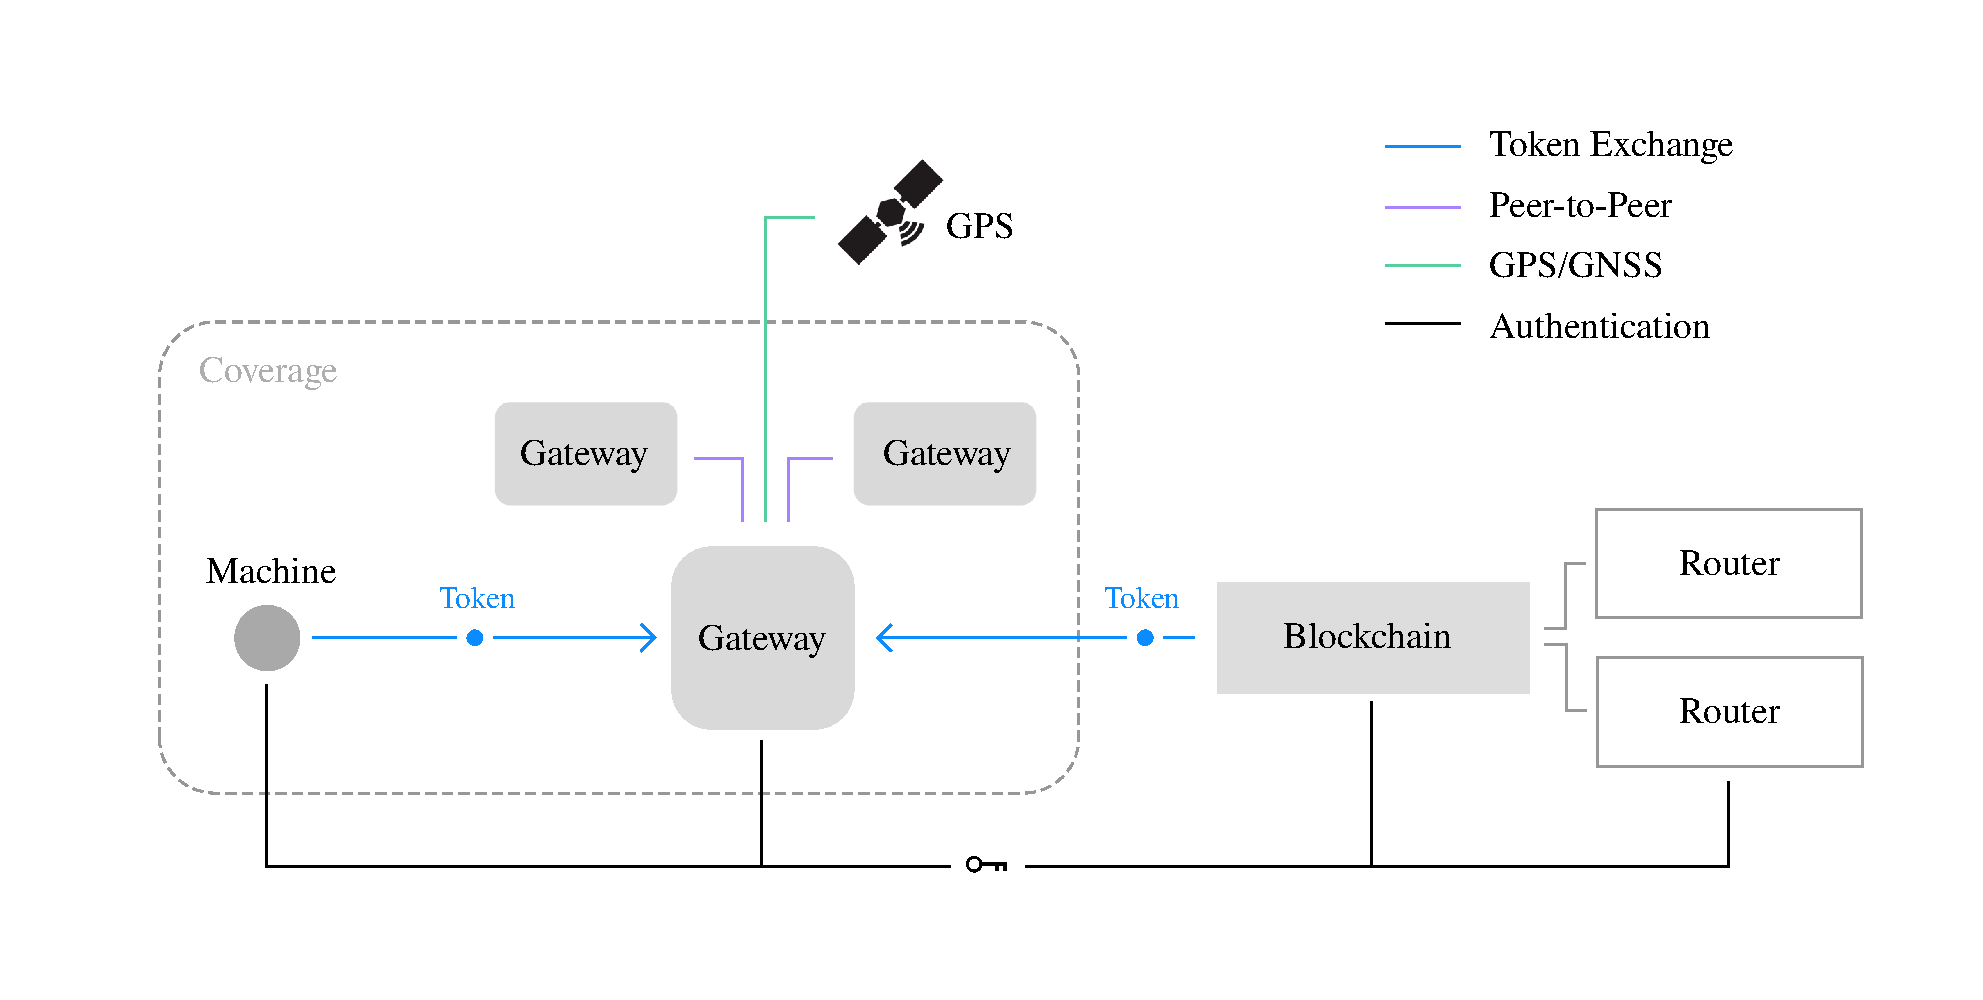
\includegraphics[width=\textwidth]{schematic.eps}
          \caption{\emph{System Overview}}\label{fig:system}
     \end{center}
\end{figure*}


\section{The Helium Peer-to-Peer Wireless Network}

We introduce the core components of the Peer-to-Peer Wireless Network.

\subsection{Participants}

There are three types of participants in the Helium network: Devices, Miners, and Servers.

\begin{description}
    \item [Devices] send and receive encrypted data from the Internet using hardware compatible with LongFi \secref{longfi}. There are hundreds of thousands of devices in the wild today capable of supporting LongFi. These devices can be updated via a firmware update to communicate with the LongFi peer-to-peer wireless network.
    \item [Miners] provide wireless network coverage to the Helium network via purpose-built hardware, called Hotspots \secref{hotspots}, which provide a long-range bridge between LongFi devices and the Internet. Users join the Helium network as Miners by purchasing or building a Hotspot that conforms to the speciification, and \emph{burning} a number of Data Credits \secref{staking}. Miners participate in the \emph{Proof-of-Coverage} \secref{poc} process to prove that they are continuously providing wireless network coverage that Devices can use. Miners join the Helium network with a score \secref{scores} that diminishes as blocks pass without valid proofs being submitted. At a given epoch, a new group of Miners are elected to an asynchronous byzantine fault tolerant \emph{consensus group} which mines new blocks. As a Miner's score drops their probability of being elected to the consensus group diminishes.
    \item [Servers] are Internet applications that purchase encrypted Device data from Miners. In locations with a sufficient number of Miners, Servers can pay several Miners to obtain enough copies of a packet to geolocate a Device without needing satellite location hardware, which we call \emph{Proof-of-Location}. Servers are the termination point for Device data encryption. Devices record to the blockchain to which Servers a given Miner should send their data, such that any Hotspot on the Helium network can send any Device data to the appropriate Server. Servers are responsible for confirming to Hotspots that Device data was delivered to the correct destination and that the Miner should be paid for their service.
\end{description}

\subsection{Blockchain} \label{blockchain}

The Helium network is a distributed ledger designed to provide a cost-effective way to run application logic core to the operation of the wireless network, store immutable Device data fingerprints, and furnish a transaction system. The Helium network is an immutable append-only list of transactions which achieves consensus using the \emph{Helium Consensus Protocol} \secref{consensus}. Users internal and external to the network have access to the blockchain, which is a new implementation built from scratch specfically for this purpose.

The blockchain consists of blocks which contain a header and a list of transactions. There are several kinds of transactions, outlined in \secref{transactions}. There is no general purpose scripting or smart contract language; all transaction types are implemented natively.

At a given epoch a block consists of:

\begin{center}
    \begin{tabular}{|c|}
         \hline
         Height \\
         \hline
         Time \\
         \hline
         HoneyBadgerBFT Round \\
         \hline
         Previous Block Hash \\
         \hline
         Transactions \emph{1..n} \\
         \hline
         Consensus Group Signatures \emph{1..n} \\
         \hline
         Election Epoch Number \\
         \hline
         Epoch Start Time \\
         \hline
    \end{tabular}
\end{center}

As the \emph{Proof-of-Coverage} \secref{poc} is valuable to the network, Miners are required to submit their proofs at regular intervals. All Miners have a score, which decays as blocks pass, and is boosted by submitting \emph{Proofs-of-Coverage} to the blockchain. At a fixed epoch, a \emph{HoneyBadgerBFT} \cite{honeybadger} consensus group of the highest scoring Miners is elected. For that epoch, all transactions are encrypted and submitted to the consensus group for inclusion in the blockchain. The consensus group is responsible for decrypting transactions using \emph{threshold decryption}, agreeing on the validity and ordering of transactions, forming them into blocks, and appending them to the blockchain.

As the consensus group is validating transactions without having to provide an associated block-proof (beyond a threshold signature), there is practically no settlement time, and the transaction throughput is extremely high compared to a \emph{Nakamoto Consensus} blockchain such as Bitcoin or Ethereum. The Helium Consensus Protocol is outlined in detail in \secref{consensus}.

\subsection{Physical Implementation}

The Helium network is also a \emph{physical} wireless network instantiation. The participants in the Helium network can be thought of as follows:

\begin{description}
    \item [LongFi] The Helium network uses a new open wireless protocol, called \emph{LongFi}. LongFi is a long-range, low-power, wireless network protocol suitable for use with commodity hardware. LongFi compatible hardware can communicate over many square miles in dense urban environments or hundreds of square miles in rural settings. LongFi compatible hardware can last for several years using standard batteries. LongFi uses strong public key cryptography with authentication occuring through the Helium blockchain, and data is encrypted end-to-end between the device and corresponding Internet-hosted server.

    \item [Hotspots] are physical network devices that provide wide-area wireless coverage and participate as Miners in the Helium network. Hotspots transmit data back and forth between Servers on the Internet and Devices while generating \emph{Proofs-of-Coverage} for the blockchain network \secref{poc}. Hotspots are manufactured using commodity components. Each Hotspot can support thousands of connected Devices, and provide coverage over many square miles.

    \item [Devices] exist in the form of hardware products that contain a LongFi-compatible radio transceiver and communicate with Hotspots on the Helium network. LongFi is designed to facilitate low power data transmission and reception, so typically Devices exist in the form of battery-powered sensors that can operate for several years using standard batteries (although mains-powered Devices also work quite well). Devices can exist in a variety of forms, depending on the product or use case, and a variety of transmission and reception strategies can be employed to optimize for transmission/reception frequency or battery life. Device manufacturers are encouraged to use hardware-based key storage which can securely generate, store, and authenticate public/private key pairs without leaking the private key.
\end{description}

In this section, we expand on the components of the wireless network.

\subsection{Wireless Protocol (\emph{LongFi})}\label{longfi}

\subsubsection{Motivation}

Several Low Power Wide Area Network (LPWAN) technologies and protocols are available today. These solutions focus on creating long-range, low-power Internet communication for sensors and other smart devices. Typically they trade throughput for range, with data rates as low as 18~bits~per~second (bps) and range measured in miles. In comparison, a typical WiFi network has significantly higher data rates but ranges limited to only a few dozen feet. Several of these new technologies, such as LoRaWAN~\cite{lora} and RPMA~\cite{rpma}, have gained good traction and there are many commercial products available compatible with these systems. While there are many open-standard wireless protocols none meet our decentralized routing, security, long range and low power criteria. It is this lack of open solutions that drove the creation of a new protocol.

\subsubsection{Outline}

We introduce \emph{LongFi}. LongFi is a highly secure, long range, low power, bi-directional wireless network protocol that is compatible with a wide range of existing radio transceivers operating in the sub-GHz unlicensed frequency spectrum. Authentication with the wireless network uses modern public-key encryption and NIST~P-256 ECC key pairs, with the public keys for all participants stored in the blockchain.

LongFi is built on the LoRa physical modulation format, which is widely supported and has excellent resistance to RF noise. There are dozens of vendors implementing radio transceivers compatible with LongFi, such as Microchip, Semtech, and HopeRF.

LongFi is a \emph{narrowband} wireless protocol which creates dozens of channels within the unlicensed spectrum and employs frequency hopping to switch between them. Typically frequency hopping requires a complex time-synchronized system that is limited in capacity. However, devices using LongFi do not need to coordinate with Hotspots on channel selection as Hotspots are capable of hearing multiple channels within the available spectrum at any time.

LongFi requires no centralized server architecture, and as such no "roaming" specification is required. Organizations deploying Devices create a special type of blockchain transaction called an \emph{Organizationally Unique Identifier (OUI)}, which issues a serialized unique identifier to the creator. Each OUI stored on the blockchain contains one or many destination protocol/address pairs. LongFi devices owned by an organization use this OUI as a prefix to their own address and includes it in the header transmitted along with every packet. Devices send encrypted data packets, but send the header unencrypted, and Hotspots inspect the blockchain to determine where those data packets should be delivered based on the OUI prefix and an inspection of the current state of the blockchain ledger. 

The full LongFi specification will be made available in Q4 2019.

\subsection{Hotspots}\label{hotspots}

Hotspots are physical network devices operated by Miners that create LongFi wireless coverage over wide areas. They transmit data back and forth between Servers on the Internet and Devices on the network, process blockchain transactions, and create \emph{Proofs-of-Coverage} for the blockchain network \secref{poc}. Hotspots can connect to the Internet using any TCP/IP capable backhaul. Each Hotspot contains radio frontend chips capable of listening to several MHz of radio spectrum at a time. Hotspots can hear any LongFi packets transmitted within the frequency range, and no channel hopping synchronization between the Hotspot and Device needs to occur. This allows Devices to remain inexpensive and relatively simple and reduces wireless protocol overhead.

Hotspots require a GPS or GNSS receiver to obtain accurate position and date/time information. This satellite-derived location is used in conjunction with other techniques to verify that a Hotspot is, in fact, providing wireless network coverage in the location it claims. Because satellite location messages are easy to fabricate and do not necessarily prove that wireless RF coverage is being created, multiple mechanisms are required to validate this work as described in more detail in \secref{poc}.

Satellite location information is also correlated with packet arrival events and can be used, in conjuction with other Hotspots who observe the same packet, to \emph{geolocate} devices that are not explicitly sending location information via GPS or some other means. This allows devices to locate themselves without requiring a GPS/GNSS transceiver, and therefore provide location data at a fraction of the battery life and cost of competing methods.

A finished Hotspot product was made available in June 2019.

\subsection{Devices}\label{devices}

A \emph{Device} is any wireless hardware capable of communicating with Hotspots via LongFi. LongFi is designed to facilitate low power data transmission and reception, so typically devices would exist in the form of battery-powered sensors that can function for several years using standard batteries.

LongFi is designed such that Devices can be manufactured using commodity hardware available from a wide variety of vendors with a very low-cost bill of materials (BOM). The technology in modern radio transceivers, such as the Semtech SX1262, enables exceptionally long-range network systems that can be built without the need for licensed spectrum operation or expensive association membership fees. Some of these radios are available for around \$1 at reasonable volumes.

It is recommended that each Device use the Microchip ECC608A or equivalent hardware-based key storage device, which can securely generate, store, and authenticate public/private \emph{NIST P-256 ECC} \cite{nist} key pairs without leaking the private key. A wide array of defense mechanisms prevent logical attacks on the encrypted data between the key storage device and its host Device, along with physical protections on the security device itself.

\subsection{Servers}

Servers are Internet-deployed applications that receive LongFi packets from Devices via Hotspots and route them to appropriate destinations such as an HTTP or MQTT endpoint.

Servers serve several functions on the Helium network, including:

\begin{itemize}
    \item Authenticating Devices with the network;
    \item Receiving packets from Hotspots and routing them to the Internet;
    \item Delivering downlink messages, including OTA updates, to Devices via Hotspots;
    \item Burning Data Credits in the name of Hotspots who routed Device data for them;
    \item Providing authentication and routing mechanisms to third-party cloud services such as \emph{Google Cloud Platform} or \emph{Microsoft Azure}; and
    \item Storing and making available a full copy of the blockchain ledger by acting as a \emph{full node} \secref{full-nodes}
\end{itemize}

When a Hotspot receives a data packet from a Device on the network, it queries the blockchain ledger to determine which Server to use given the Device's OUI. Anyone is free to host their own Server and define their Devices' traffic to be delivered there by any Hotspot on the Helium network by creating an OUI transaction. This ability allows users of the Helium network to create VPN-like functionality whereby encrypted data is delivered only to a Server (or set of Servers) that they specify and can optionally host themselves.

Routers can implement a system called a \emph{Channel} which handles the authentication and routing of data to a specific third party Internet application, such as \emph{Google Cloud Platform IoT Core}. These Channel implementations can take advantage of a Device's onboard hardware security to create a secure, hardware-authenticated connection to a third party which would otherwise be difficult to implement directly on an embedded microcontroller. We will make available an open source reference implementation of a Channel that can be used to build additional interfaces to Internet services.

Helium Inc hosts a high-availability cloud Server for anyone to use and also provides and maintains an open-source Server that is available either as source code or a binary package for a variety of operating systems and distributions.

The protocol specification required for implementing a Server is defined in the LongFi Wireless Specification document that will be made available in Q4 2019.

\section{\emph{Proof-of-Coverage}}\label{poc}

In the Helium network, Miners must prove that they are providing wireless network coverage that Devices are able to use to communicate with the Internet. Miners do this by complying with the \emph{Proof-of-Coverage} protocol which the Helium network and other Miners audit, verify and use to obtain cryptographic proof of dishonest behavior. With \emph{Proof-of-Coverage} we can obtain cryptographic proof of the approximate location and time of events occurring within the Helium network.

\subsection{Motivation}

Most existing blockchain networks such as Bitcoin~\cite{bitcoin} and Ethereum~\cite{ethereum} use a \emph{Proof-of-Work} system that relies on an algorithmic puzzle that is asymmetric in nature. These proofs are extremely difficult to generate, but simple for a third party to verify. Security on these networks is achieved by the network-wide \emph{consensus} that the amount of computing power required to generate a valid proof is difficult to forge, and as subsequent blocks are added to the blockchain, the cumulative difficulty of the chain becoming prohibitively difficult to fabricate.

The proofs used in the Helium network must be resistant to \emph{Sybil attacks} in which dishonest Miners create pseudonymous identities and use them to subvert the Helium network and gain access to mining rewards to which they should not be entitled, and \emph{Eclipse attacks}, where an attacker attempts to isolate a network participant and subsequently prevent their target from attaining a true picture of real network activity and the current ledger state. These attack vectors are particularly difficult to manage in a network deployed via broadly distributed commodity hardware.

We later propose the Helium Consensus Protocol \secref{consensus} that uses \emph{Proof-of-Coverage} to both secure the blockchain and provide an extremely useful service to the Helium network, which provides wireless network coverage that Devices can use to send data to and from the Internet.

\subsection{Inspiration}

\emph{Proof-of-Coverage} is a novel proof that allows Miners to prove that they are providing wireless network coverage in a specific region to a challenger. Proof-of-Coverage is an interactive protocol where a set of targets assert that wireless coverage exists in a specific GPS location, and then convinces the challenger via a cryptographic receipt system that the coverage does in fact exist. Proof-of-Coverage is the first such protocol that attempts to prove the veracity of miners in a physical space, and then use the results to achieve consensus on a blockchain network.

With Proof-of-Coverage we aim to solve for the following:

\begin{itemize}
    \item Prove that Miners are operating RF hardware and firmware compatible with LongFi;
    \item Prove that Miners are located in the geography they claim by having them communicate via RF; and
    \item Correctly identify which version of reality is correct when there is a conflict
\end{itemize}

\emph{Proof-of-Coverage} is inspired by the \emph{Guided Tour Protocol (GTP)}~\cite{gtp} which devises a system for denial of service prevention by requiring a client to make a request to a variety of ``tour guide'' computers in order to gain access to a server. The tour guides must be visited in a specific order and a hash of data exchanged which reveals the location of the next tour guide computer in order. Only after every tour guide has been visited can the client gain access to the server.

Once the client gets to the last stop of the tour, it submits evidence of the first and last stop to the server who is able to verify that the first and last stops of the tour are correct without needing to contact the tour guides, and that the client could only know the first and last stops if it had completed the tour correctly.

While an extremely clever and innovative system, GTP is not directly suitable as a proof in the Helium network as RF networking has limited range and therefore cannot communicate with peers anywhere on the Helium network. We aim to construct a proof loosely based on the ideas presented in GTP, but applicable to our protocol.

\subsection{Constructing \emph{Proof-of-Coverage}}

With the Proof-of-Coverage protocol, we aim to construct a proof that takes advantage of the following characteristics of radio frequency (RF) communication that are unique and different to Internet communication:

\begin{enumerate}
    \item RF has limited physical propagation and, therefore, distance;
    \item The strength of a received RF signal is inversely proportional to the square of the distance from the transmitter; and
    \item RF travels at the speed of light with (effectively) no latency
\end{enumerate}

Our goal is to verify whether Miners in a physical region are acting honestly and creating wireless network coverage compatible with LongFi. To do this, a challenger $C$ deterministically constructs a multi-layer data packet $O$ which begins at an initial target, $T_1$, and is broadcast wirelessly to a set of sequential targets, $T_n$, each of which are only able to decrypt the outer-most layer of $O$ if they were the intended recipient. Each target signs a receipt, $K_s$, delivers it to $C$ and broadcasts it for the next target. Essentially an ``envelope of envelopes'' only decipherable by the intended recipient.

\begin{figure}[ht]
    \begin{center}
          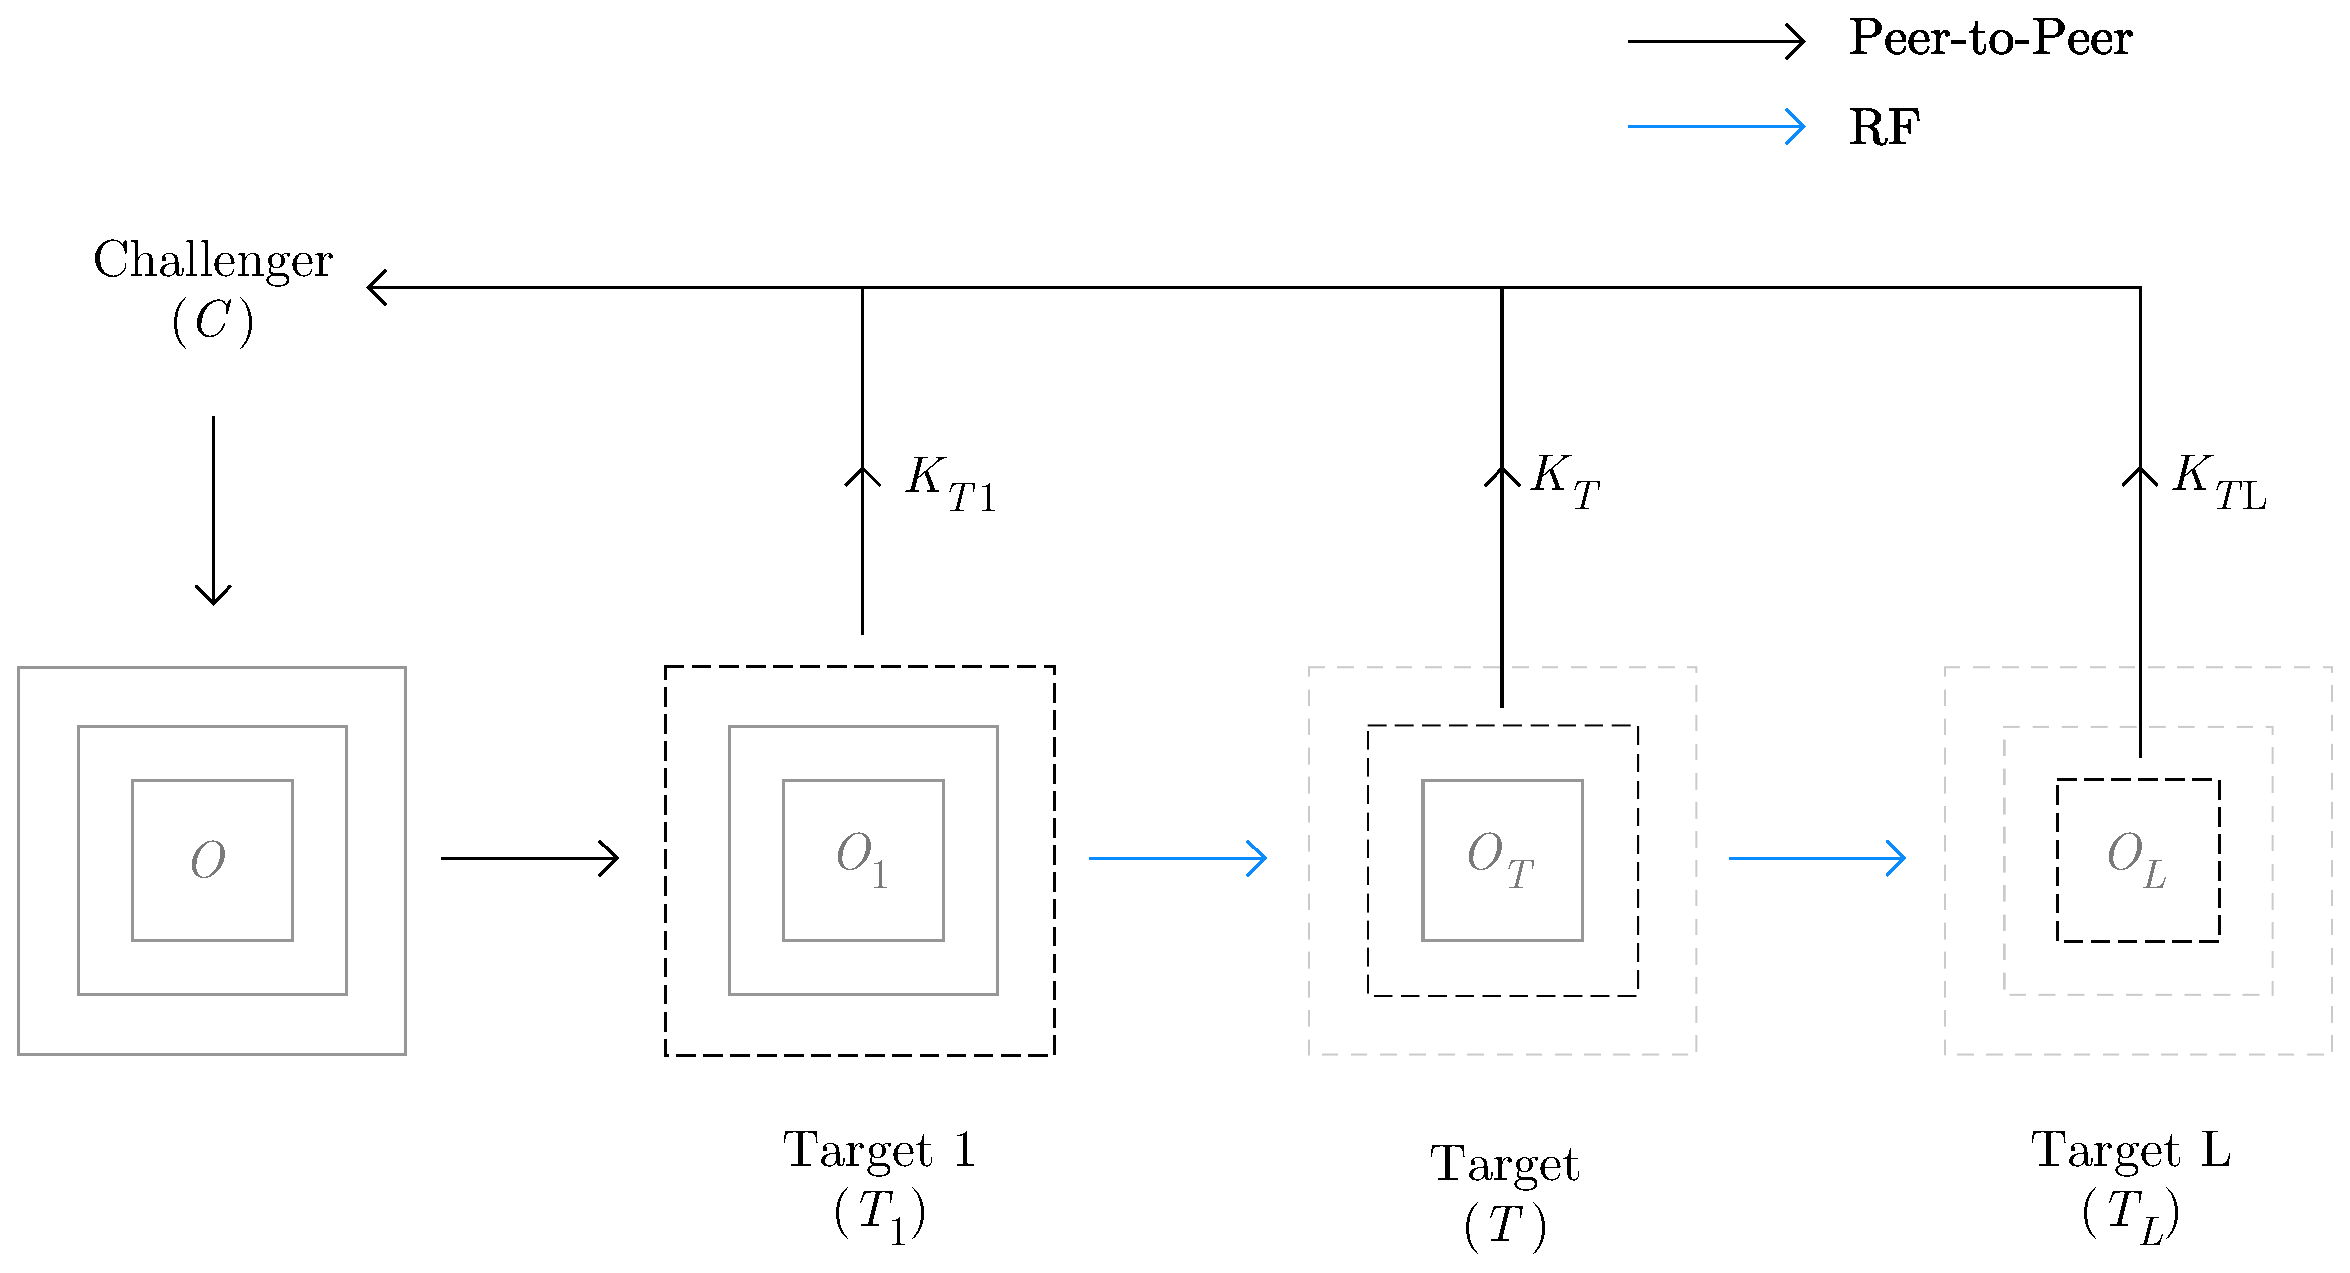
\includegraphics[width=\columnwidth]{deconstruction.eps}
          \caption{\emph{Multi-Layer Data Packet Deconstruction}}\label{fig:poc-deconstruction}
     \end{center}
\end{figure}

\subsubsection{Selecting the Initial Target}

We aim to deterministically locate a geographic reference target, $T$, for the challenger, $C$. Both $C$ and $T$ are Miners in the Helium network. $T$ does not need to be geographically proximate to $C$. To locate $T$, $C$ initially seeds verifiable entropy, $\eta$, into the selection process by signing the current block hash with its private key. Since the probabilities associated to each miner form a discrete probability distribution \eqref{eq:target-selection-probability}, $C$ uses the probability associated to each eligible Miner to locate $T$ and applies an inverse cumulative distribution function using a uniform random number generated via $\eta$. This allows us to ensure that we always target potentially dishonest Miners as they have a lower score, thus increasing their probability of being targeted by $C$. Given that a Miners score is diminishing linearly over time \secref{scores}, it is necessary to create this inverse relationship to give low-scoring Miners an opportunity to participate in the process and increase their score. This diminishing score also incentivizes all the participants to participate in the process.

\subsubsection{Constructing the multi-layer challenge}

Once $T$ has been selected, $C$ must construct the multi-layer challenge packet, $O$. $O$ is a data packet broadcast wirelessly using LongFi and received by geographically proximate targets $T_n$. Geographically proximate is defined as within a radius of $T$, a network value $T$\textsubscript{radius} initially set at 1 mile. Each layer of $O$, $O_l$, consists of a three-tuple of $E\left(S, \psi, R\right)$, where $E$ is a secure encryption function using the Elliptic-Curve Diffie-Hellman (ECDH) derived symmetric key, $S$ is a nonce, $\psi$ is the time to broadcast the next layer of the challenge and $R$ is the remainder of $O$ consisting of recursive three-tuples. The maximum number of layers $O_l$ is bounded by a network value, $O$\textsubscript{max}, initially set at 7.

The construction logic of $O$ by $C$ is as follows:

\begin{enumerate}
  \item A set of candidate nodes, $T_n$, are selected such that all members of $T_n$ are within a contiguous radio network that also contains $T$;
  \item Two targets, $T_1$ and $T_L$, are selected by finding the highest scoring targets in $T_n$ furthest from $T$;
  \item A weighted graph, $T_g$, is constructed from $T_n$ such that members of $T_g$ in radio range of each other are connected by an edge weighted by the value of \(1 - \Big({score(T_a) - score(T_b)}\Big)\);
  \item The shortest path between $T_1$ to $T$ to $T_L$ is computed using Dijkstra's algorithm\cite{dijkstra} using the edge weights from the previous step;
  \item An ephemeral public/private keypair $E_k$ and $E$\textsubscript{k-1} are generated;
  \item A layer $O_l$ is created and added to $O$, and $S$ is encrypted with the combination of the public key of $T_L$, retrieved from the blockchain as $T_L$$_k$ and $E$\textsubscript{k-1} as an ECDH exchange to compute a shared secret, known only to both parties $C$ and $T_L$; and
  \item The previous step repeats with additional layers added to $O$ until all $T_L$ $\rightarrow$ $T_1$ have a layer $O_l$ included in $O$
\end{enumerate}

The resulting $O$ can be visually represented as depicted in \figref{fig:poc-o_construction}.

\begin{figure}[ht]
    \begin{center}
          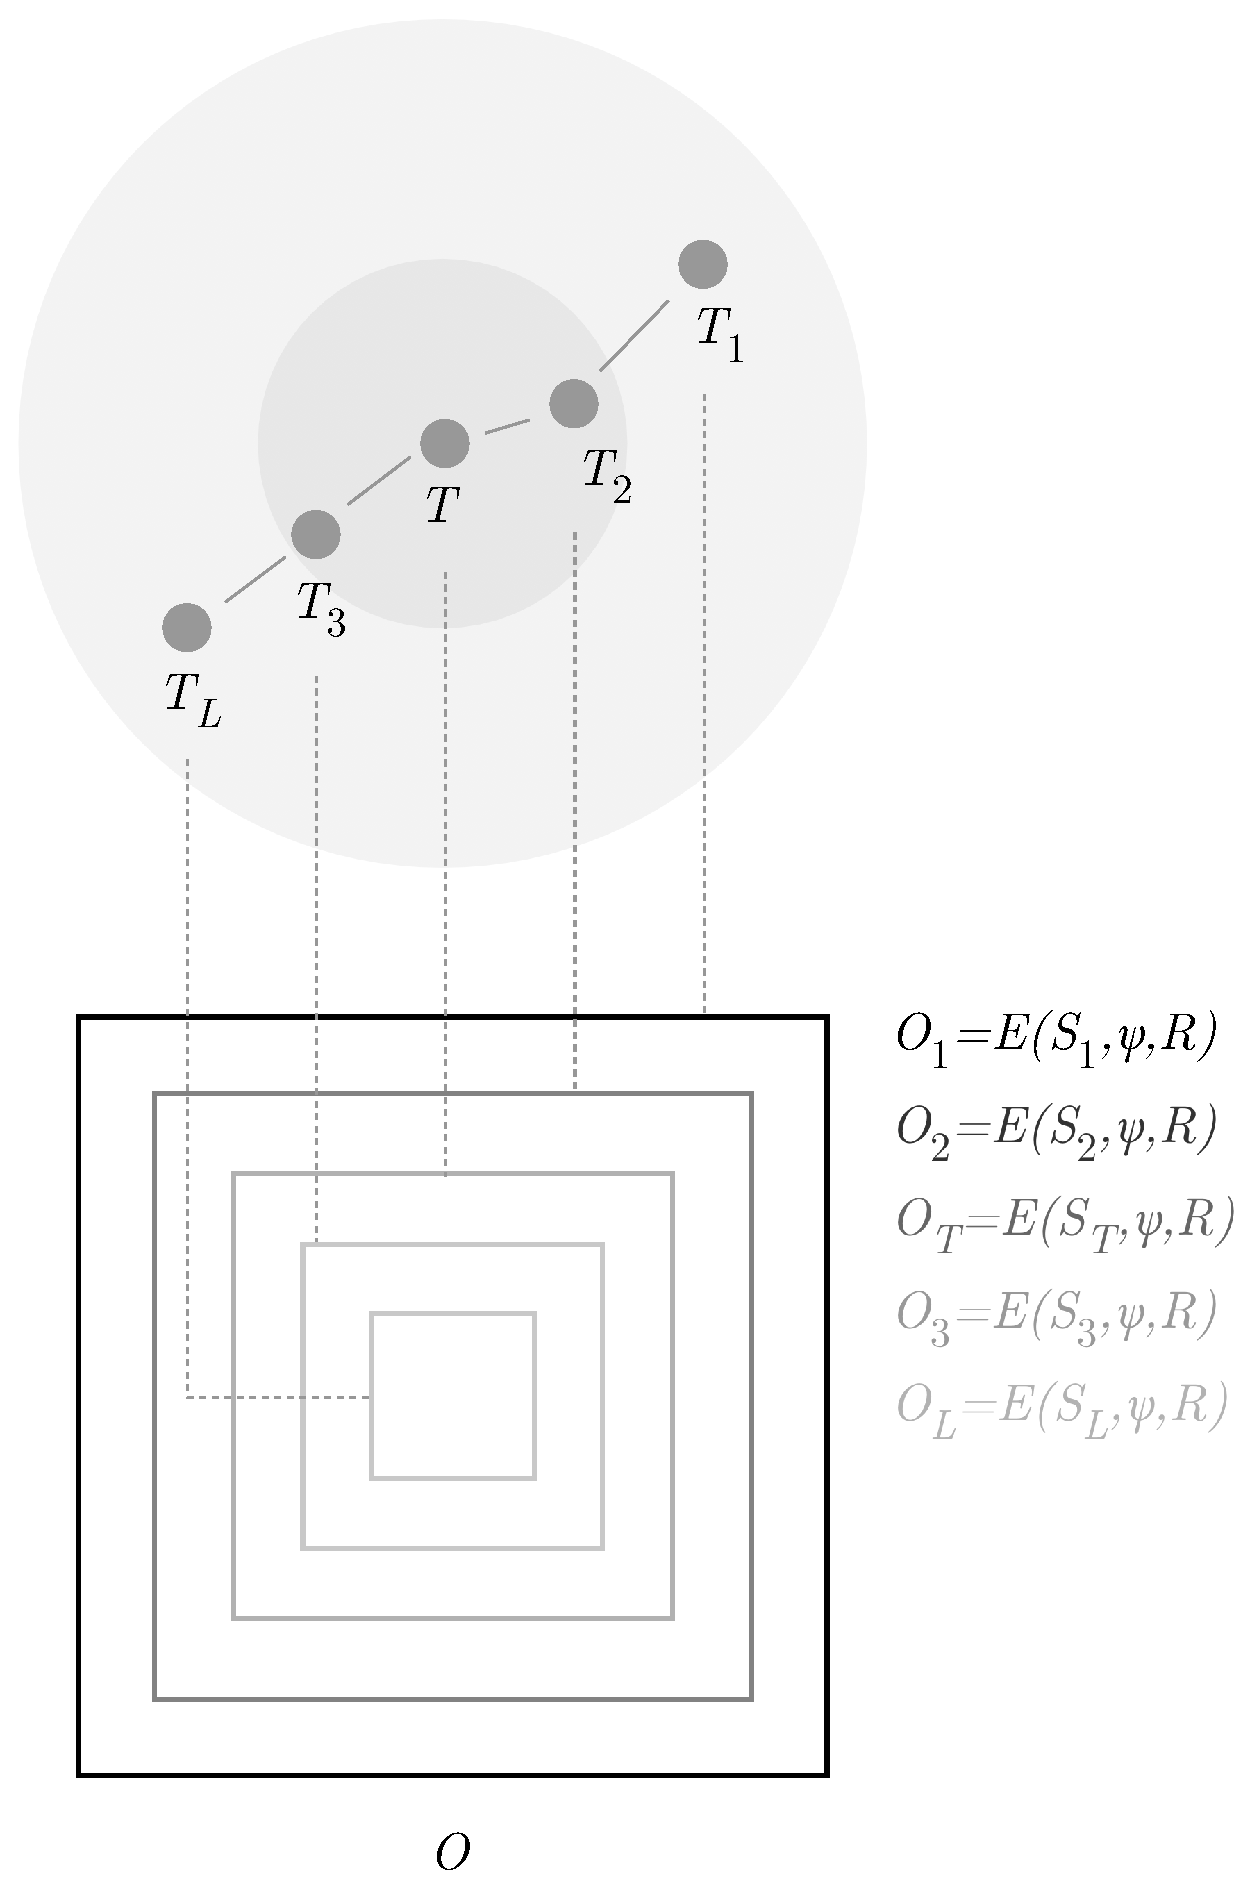
\includegraphics[width=\columnwidth]{o_construction.eps}
          \caption{Construction of $O$}\label{fig:poc-o_construction}
     \end{center}
\end{figure}

\subsubsection{Creating the Proof}

Once $O$ has been constructed, it is delivered to $T_1$ via the peer-to-peer network and immediately broadcast by $T_1$ via the LongFi network. LongFi is not a point-to-point system, so several Miners within proximity of $T_1$ will hear $O$. In this example, only the specific target $T$ will be able to decrypt $E$ and send a valid receipt back to the challenger, $C$.

We describe the approximate flow of \emph{Proof-of-Coverage} creation as follows:

\begin{enumerate}
  \item $T_1$ receives $O$ from $C$ via the peer-to-peer network, decrypts the outermost layer and immediately broadcasts it $R$ via the LongFi network;
  \item $T$ hears $O$ and attempts to decrypt the value of $E$ by using its private key where $pk:\ E_{pk}\left(S, \psi, R\right)$;
  \item $T$ records both the time of arrival $\beta$ and the signal strength $\upsilon$ of $O$;
  \item If successful, $T$ then creates signed receipt $K_s$, where \\${K_s = \left(S || \beta || \upsilon\right)}$ signed by the private key of $T$;
  \item $T$ submits $K_s$ to $C$ via the peer-to-peer network, and broadcasts $O$ via LongFi; and
  \item These steps repeat for $T_1$..$T$..$T_L$, with $T_L$ being the last target in the graph
\end{enumerate}

$C$ expects to hear responses from $T_g$ within a time threshold $\lambda$, otherwise it considers the \emph{Proof-of-Coverage} to have concluded. Because $C$ is the only party with complete knowledge of $O$, upper bounds of the values for $\beta$ and $\upsilon$ are assigned by $C$ which are used to verify that each layer of $O$ was transmitted approximately where and when it was expected. The upper bound for $\beta$ is limited by the speed of light $\tau$ between $T_n$ and $T_n-1$. Thus we know that, subject to some slight delays from reflection or multipath, the packet should not arrive at $T_g$ later than $\tau$ multiplied by the geographical distance $D$ plus some small episilon value, $\upsilon = \tau \times \Big(D + \epsilon\Big)$. For $\upsilon$, because of the inverse-square law, we can calculate the maximum RSSI (Received Signal Strength Indication) possible for a packet transmitted, $\mu$, from $T_g-1$ to $T_g$ as $\mu = \frac{1}{D^2}$. Hotspots that are closer than expected, or which are transmitting at a higher power to mask their location disparity, are unlikely to get $\mu$ correct, given that they do not know who the next layer of $O$ is addressed to.

Once $T_L$ has delivered receipt to $C$, or $\lambda$ has elapsed, the \emph{Proof-of-Coverage} is completed. The collection of signed receipts, $K_s$, constitute the \emph{Proof-of-Coverage} that $C$ will submit to the Helium network.

\begin{figure}[ht]
    \begin{center}
          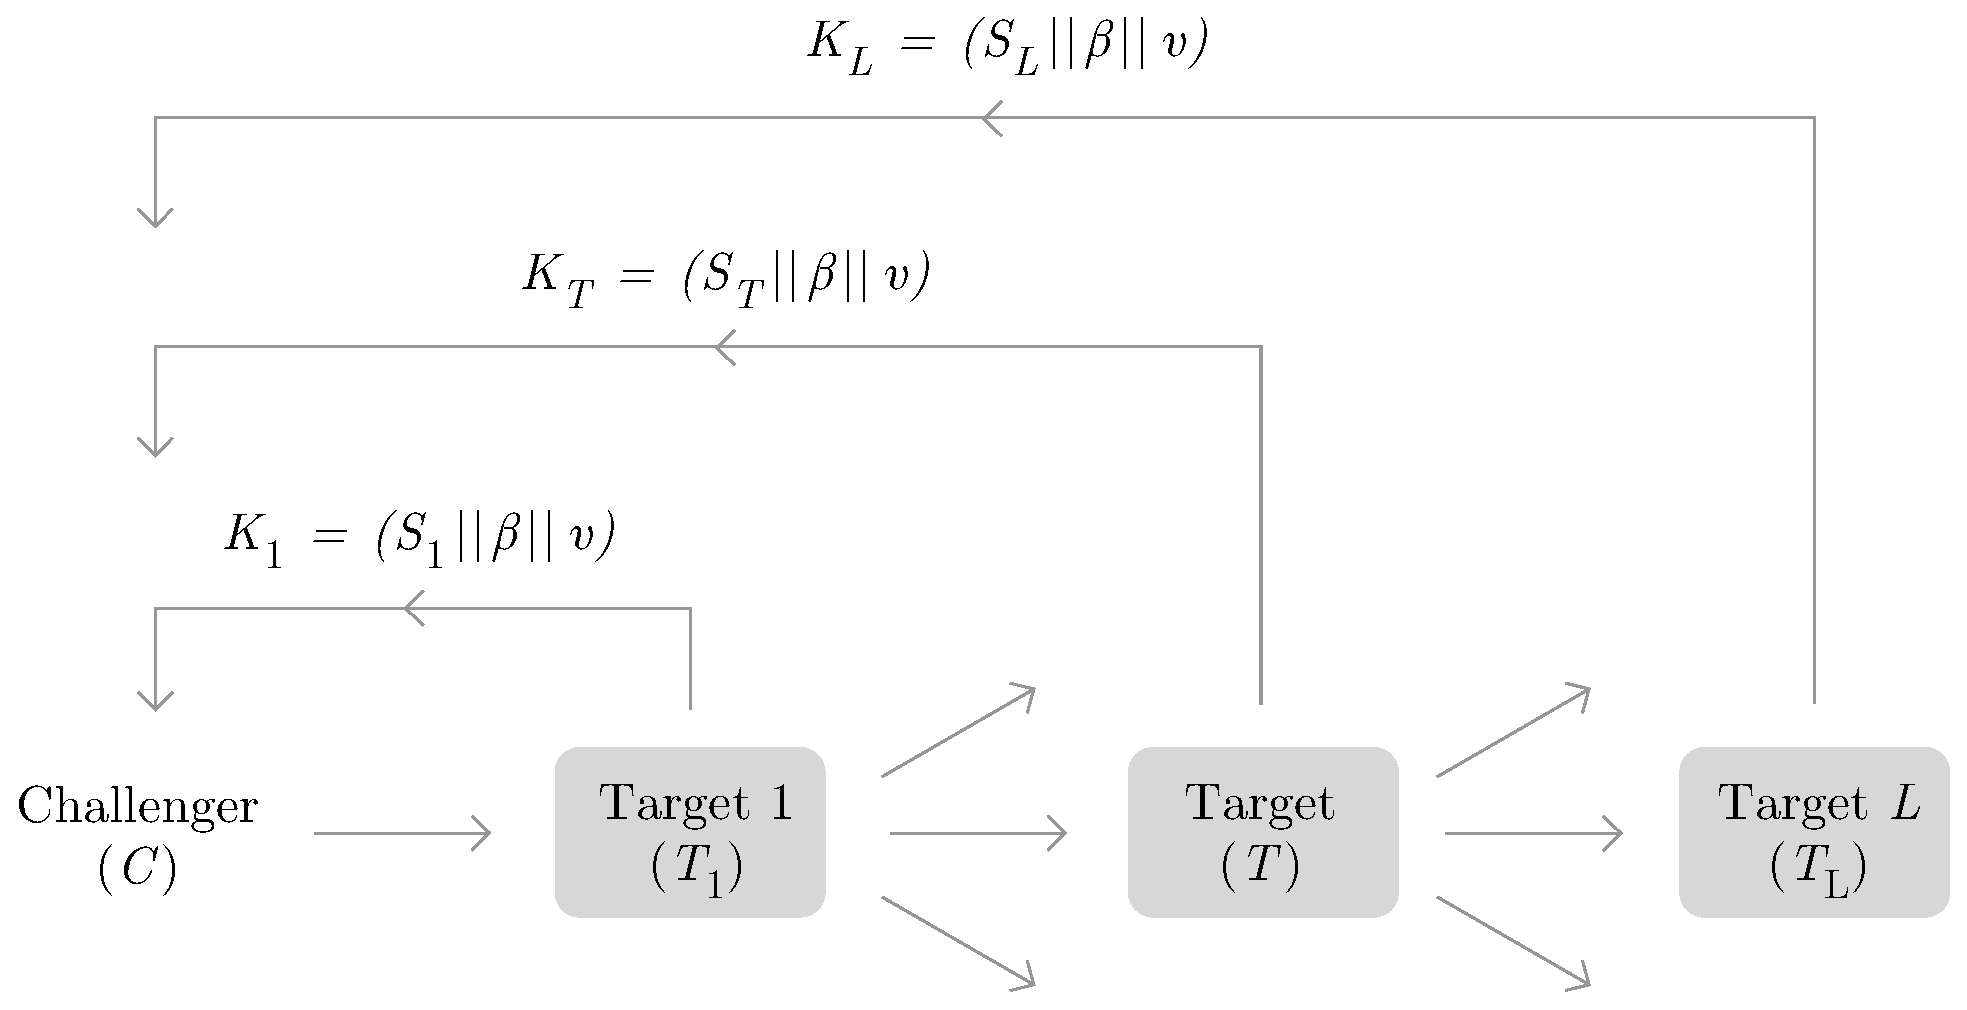
\includegraphics[width=\columnwidth]{o_propagation.eps}
          \caption{\emph{Proof-of-Coverage} flow}\label{fig:poc-propogation}
     \end{center}
\end{figure}

\subsubsection{Witnesses}

\todo{EXPLAIN MORE ABOUT HOW WITNESSES WORK HERE}

\subsubsection{Scoring}\label{scores}

The score allocated to a Miner, and therefore the resulting score of the \emph{Proof-of-Coverage}, is an integral part of the Helium Consensus Protocol described in \secref{consensus}. When Miners join the Helium network, they are assigned a score, $\phi_m$. We consider any Miner with a score greater than $\phi_m$ to be an \emph{honest miner}. This score depreciates according to the number of verifications the Miner has as well as the height since its last successful verification. As $\phi_m$ decreases the probability of the Miner $M$ being the target for $C$ increases, such that the Helium network continually attempts to prove that the lowest scoring Miners are acting honestly, and giving Miners a reasonable chance to improve their scores.

In order to achieve this behavior we define the following invariants:

\begin{tabular}{l l}
        $M$, & Miner                                         \\
        $v$, &number of successful verfications for $M$ -\\
        & number of failed verifications for $M$ \\
        $h$,          & height since the last successful verification for $M$\\
\end{tabular}

If we assume that the ideal verification interval for any Miner is close to 240 blocks (4 hours if we assume a 60 second block time), we scale these invariants to fit the scoring functions:

\begin{tabular}{l l}
        $v'$, &$v/10.0$\\
        $h'$, &$h/480$ \\
\end{tabular}

Using the above we can now construct a staleness-factor, $\delta$, which would be used in determining the score of the Miner $M$.

\begin{equation*} \label{eq:equation:score1}
        \delta{m} = \begin{cases}
        	-(8.h')^{2}&\text{$v'$ = 0}\\
        	v'.(1 - \frac{h'^{2}}{min(0.25, v')})&\text{$v'$ $>$ 0}\\
        	v'.(1 - 10.v'.h'^{2})&\text{$v'$ $<$ 0}
        \end{cases}
\end{equation*}

The above conditions strictly adhere to the following principles:

\begin{enumerate}
  \item A negative $v$ indicates that the Miner is consistently failing verification.

  \item If $v$ = 0, then we do not have any trust information, therefore, we use a steep parabolic curve for the decay dependent on $h'$.

  \item If $v$ $>$ 0, then it implies that the Miner has been successfully verified consistently, hence, we use an inverse parabolic curve that crosses the Y axis at 1, where the width of the parabola increases as a factor of $v$ up to 0.25. This implies that the more positive verifications \secref{poc} the Miner has accrued, the slower its score decays as a factor of $h'$.

  \item Finally, if $v$ $<$ 0, then this is the inverse of the above case, wherein, a Miner has consistently been failing verification. Therefore, we use a similar parabola as above; however, the width of the parabola decreases as a factor of $v$, leading to a higher score decay for the Miner as a factor of $h'$.

\end{enumerate}

\figref{fig:score-trends} shows the trends for each of the above functions.

\begin{figure}[ht]
    \pgfplotsset{width=7cm, compat=newest}
    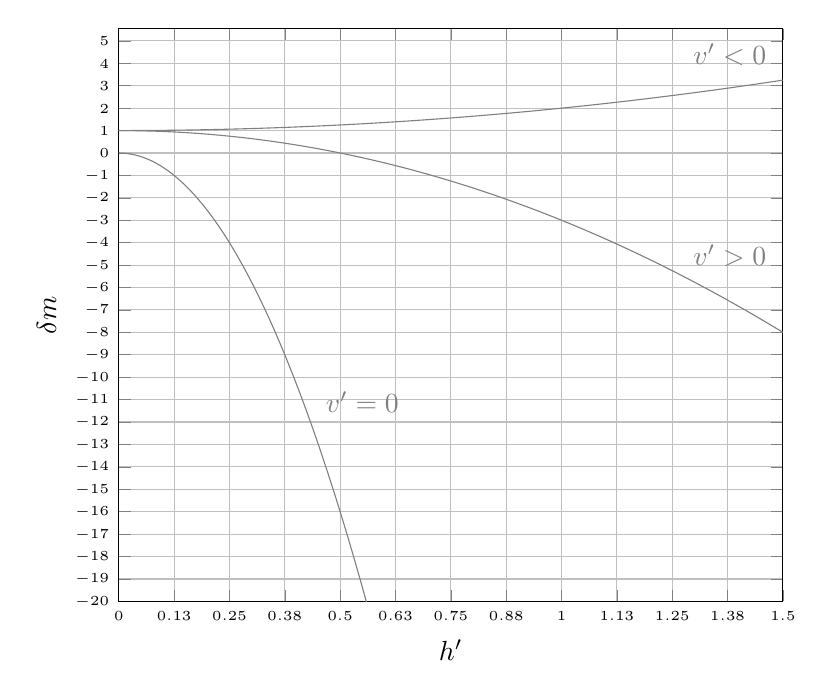
\begin{tikzpicture}
        \begin{axis}[xlabel = $h'$,
        ylabel = $\delta{m}$,
        xmin=0,
        xmax=1.5,
        ymin=-20,
        xtick={0, 0.125,...,1.5},
        ytick={-20, -19,...,5},
        scale only axis,
        grid=major,
        tick label style={font=\tiny}]
            \addplot[smooth, color=gray, samples=500]{-(8*x)^2};
            \node [anchor=south, color=gray] at (axis cs:0.55, -12)  {$v'=0$};
            \addplot[smooth, color=gray, samples=500]{1 -((x)^2)/0.25};
            \node [anchor=south, color=gray] at (axis cs:1.38, -5.5)  {$v'>0$};
            \addplot[smooth, color=gray, samples=500]{1 +((x)^2)};
            \node [anchor=south, color=gray] at (axis cs:1.38, 3.5)  {$v'<0$};
        \end{axis}
    \end{tikzpicture}
    \caption{\emph{Trendlines for the scoring functions}}\label{fig:score-trends}
\end{figure}

Adhering to the above set of rules, we define the following scoring function, which is essentially a variation of a sigmoid curve fluctuating between values (0, 1):

\begin{equation*} \label{eq:equation:score2}
        \phi_m = \frac{\arctan(2.\delta{m}) + 1.58}{3.16}
\end{equation*}

This scoring function yields \figref{fig:score-stale}, which shows the variation of the score with the staleness-factor:

\begin{figure}[ht]
    \pgfplotsset{width=7cm, compat=newest}
    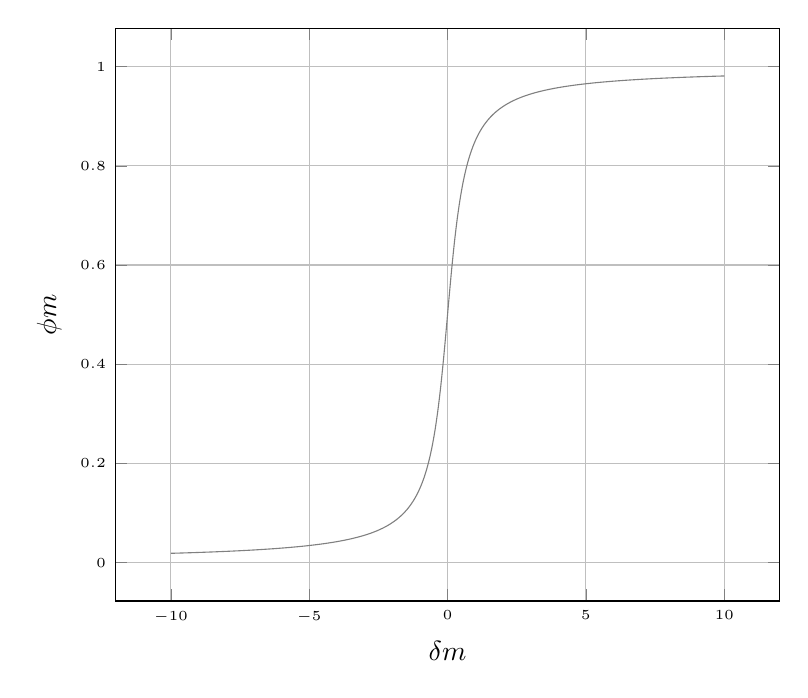
\begin{tikzpicture}
        \begin{axis}[xlabel = $\delta{m}$, ylabel = $\phi{m}$,
        scale only axis,
        grid=major,
        tick label style={font=\tiny}]
            \addplot[smooth, color=gray, domain=-10:10, samples=200]{(1.58 + rad(atan(2*x)))/3.16};
        \end{axis}
    \end{tikzpicture}
    \caption{\emph{Scoring algorithm and the resulting staleness factor}}\label{fig:score-stale}
\end{figure}

\figref{fig:score-graph} shows a snapshot of a random subset of the Helium network at any blockchain height \textit{h}. The Miners represent random locations with an illustrated score, while the edges are calculated using Dijkstra's algorithm\cite{dijkstra}.

\begin{figure}[ht]
    \begin{center}
          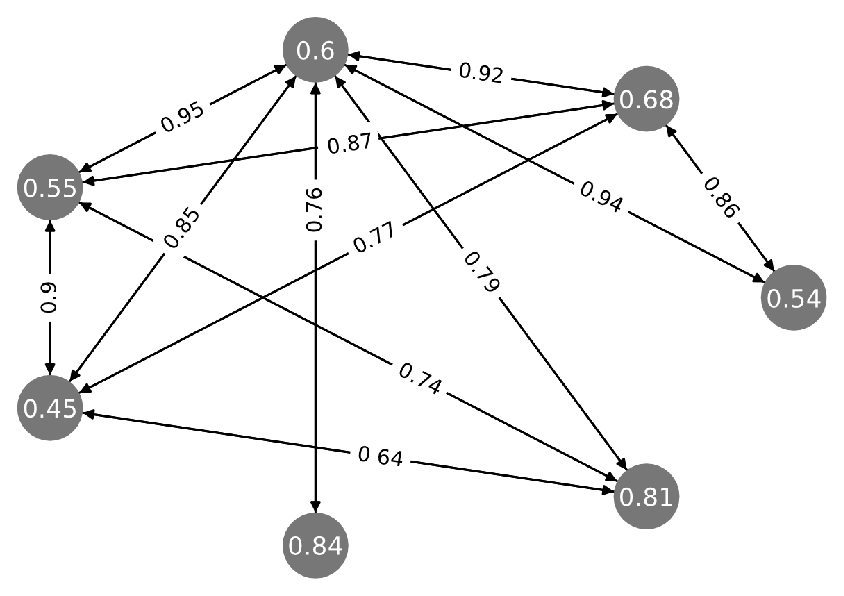
\includegraphics[width=0.8\columnwidth]{chart.eps}
          \caption{\emph{Snapshot of a random subset of the initial network}}\label{fig:score-graph}
     \end{center}
\end{figure}

After 10,000 iterations the Helium network appears as represented in \figref{fig:score-graph10000}.

\begin{figure}[ht]
    \begin{center}
          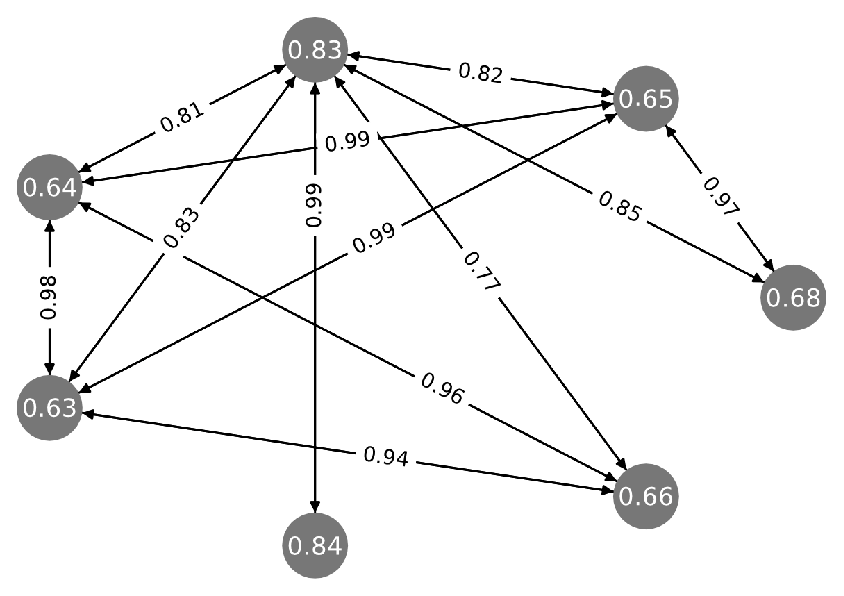
\includegraphics[width=0.8\columnwidth]{chart1000.eps}
          \caption{\emph{Snapshot of a random subset of the network after 10000 iterations}}\label{fig:score-graph10000}
     \end{center}
\end{figure}

The goal of this system is to ensure that the scoring algorithm considers that some Miners may attempt to act dishonestly. However, because the calculated edge-weights (via Dijkstra's algorithm) and the target selection mechanism ensure that we only boost the score of a Miner when it is being verified by other high scoring Miners, we believe that the system will favor legitimate Miners and deter dishonest ones.

\subsubsection{Target Selection}

Due to the way scoring decays, there is a possibility that a given Miners' score may become stale as that Miner may not be verified within a reasonable interval. We therefore structure the target selection mechanism to give Miners a statistically greater chance to increase their score by being selected as a target as their score decays. This is accomplished by biasing the probability of Miners being selected as potential targets based on their individual scores.

Let the set of miners be defined as:
\begin{equation*} \label{eq:set-of-miners}
        N = \{m_1, m_2, m_3 \dots\ m_n \mid n > 1\}
\end{equation*}

Let the set of miner scores be defined as:
\begin{equation*} \label{eq:set-of-scores}
        S = \{\phi_m, m \in N\}
\end{equation*}

We assign the target selection probability to each miner in the following way:
\begin{equation} \label{eq:target-selection-probability}
        P(m) = \frac{1-\phi_m}{n - \displaystyle\sum_{i=1}^{n} {\phi_{m_i}}}
\end{equation}

The above equation ensures that the Miner with the lowest score is assigned the highest probability of being selected as a potential target while the opposite holds for the Miner with the highest score.

Furthermore, it also asserts that the probabilities are inversely proportional to the score of an individual Miner. This allows us to successfully target potentially low scoring Miners and improve the overall balance of the scoring system.

Another valuable aspect of assigning the probability as shown above is that all the probabilities together form a discrete probability distribution. A discrete probability distribution satisfies the following equation:

\begin{equation*} \label{eq:discrete-probability-distribution}
        \sum_i P(M=i) = 1
\end{equation*}


\subsubsection{Verifying the Proof}

Once $T_L$ has delivered $K_s$, or $\lambda$ has elapsed, the \emph{Proof-of-Coverage} is considered complete. When $C$ submits this proof, via a receipt transaction, all receipts $K_s$ from $T_1$...$T_L$ are included in the transaction published to the Helium network. As all the steps originally completed by $C$ are deterministic in nature with verifiable and recreatable randomness, it is simple for a verifying Miner, $V$, to recreate the original steps and verify that the proof is legitimate.

Verifying Miners in the consensus group \secref{consensus} who see the receipt transaction are able to verify the \emph{Proof-of-Coverage} by recreating the following steps:

\begin{enumerate}
        \item The verifying Miner, $V$, reconstructs the set of Miners $N$;
        \item The random seed $\eta$ can be verified by $V$ to have been created at approximately the correct time by the private key of $C$;
        \item $V$ then selects $T$ from $N$, as seeding with $\eta$ will result in the same target selection;
        \item The set of candidate $T_n$ are reconstructed from which $T_1$ and $T_L$ are determined;
        \item Dijkstra's algorithm is used to reconstruct the graph $T_g$; and
        \item The $K_s$ receipts contained in $B_C$ are verified to have been signed by the private keys of $T_1$..$T$..$T_L$
\end{enumerate}

Assuming these steps are completed successfully, the \emph{Proof-of-Coverage} is verified the scores of $T_n$ are adjusted appropriately.

\section{Token System}\label{tokens}

The Helium network uses the Burn-And-Mint Equilibrium (BME) model \ref{burnandmint} originally pinoeered by Factom \ref{factom}. 

\subsection{Understanding Token Velocity}

The vast majority of blockhain networks use utility tokens that also act as proprietary payment currencies. Each of these cryptocurrencies is presenting itself as a freestanding monetary base. Monetary bases should be valued using the equation of exchange: $MV = PQ$. Therefore $M = PQ/V$.

The V in the equation of exchange is a problem for most proprietary payment currencies. Proprietary payment currencies are, generally speaking, susceptible to the velocity problem, which will exert perpetual downwards price pressure. Due to this effect, we would expect to see utility tokens that are just proprietary payment currencies exceed a velocity of 100. As a point of reference, the USD M1 supply has a velocity of 5.5.

We can say that an asset has a velocity of 0 if, over some period of time, no one buys or sells it. The lack of liquidity would cause the asset to trade at a discount to its “intrinsic” value. Assets need some velocity to achieve their full intrinsic value. The difference is known as the liquidity premium.

In the case of a proprietary payment token that nobody wants to hold, velocity will grow linearly with transaction volume. Per the second equation above, transaction volume could grow a million-fold and network value could remain constant. Almost all utility tokens suffer from this problem.


In the BME model thtokens are a proprietary payment currency. But unlike traditional proprietary payment currencies, users who want to use a service do not directly pay a counterparty to use the service. Rather, users burn tokens.





\section{Transactions}\label{transactions}

Transactions in the Helium network provide functionality that enables address-to-address transfers of protocol tokens, similar to many existing blockchain networks, but also provide a set of primitives that enable core functionality for the wireless network. We will first address Helium's need for microtransactions and propose a new solution.

\subsection{Types of Fees in Helium}

In this section we outline the types of fees needed on the Helium network, and propose solutions that take advantage of the unique characteristics of the Helium Consensus Protocol \secref{consensus}.

\subsubsection{Transport Fees}

Devices using the Helium network to send and receive data to and from the Internet must pay Miners what is known as a \emph{transport fee}. This fee compensates the Miner for delivering data packets between the Device and the intended router on the Internet, and is unrelated to the \emph{transaction fee} that Miners earn for mining transactions as part of blocks that are recorded to the blockchain. The fee is negotiated between the Router to which the Device belongs, and the Miner, as Devices are not directly connected to the blockchain.

Miners set the price they are willing to accept to transport data to and from the Internet on a per-byte basis.

A Devices router pays Miners the transport fee on transmission or reception of the data. This means that the Miner will receive the transport fee prior to the transaction being mined in a block and recorded into the blockchain. This entails some risk for the Miner, as they must believe that the transport payment is not malicious or fraudulent prior to it being confirmed in the blockchain. However, given how low the per-byte transport amount is likely to be, this risk seems tolerable. A Miner can \emph{blacklist} a Device or organization address if they continually abuse the system.

An example transport fee process is as follows:

\begin{enumerate}
  \item A Miner, $M$, hears a packet, $P$, broadcast by Device $D$;
  \item $M$ uses the address of $D$, attached to $P$, to identify a router, $R$, as the owner of $D$;
  \item $M$ sends the signature, $K(P)$, of $P$ and an offer of $n$ tokens for transport to $R$;
  \item $R$ receives $K(P)$ and the payment offer and determines if it accepts the packet for the offered price,
  \item Assuming $R$ accepts the packet at the offered price, it constructs a transaction $T$ of value $n$ payable to $M$ and sends it to the Miner; and
  \item Once $M$ sees the transaction in the reply it delivers $P$ to $R$ and submits $T$ to the consensus group for inclusion in the Helium network
\end{enumerate}

\subsubsection{Transaction Fees} \label{fees}

Transaction fees are an essential part of most blockchain implementations. They incentivize Miners to include a transaction in their draft block and ensure that spam transactions do not pollute the Helium network.

To determine the appropriate fee for a new transaction, the transactor will take the median of the past $\delta$ packet transport fees, within some margin of error. Until $\delta$ packet transports have occured on the Helium network, the fee will be fixed at a constant value $\alpha$. By anchoring the transaction fee to the current fees being charged for transport on the Helium network, we root them in reality. The Helium network's primary purpose is to facilitate a network of wireless Internet coverage. In order to accomplish this in the long term, all of the economics of the system must align to make it practical for the primary users to transact on the Helium network. If one set of fees were to outstrip the others, then the Helium network would quickly lose its utility for the key user segment.

To enable Miners and other light clients to determine an appropriate fee, full nodes \secref{full-nodes} will expose a fee suggestion API. This way resource constrained entities that do not maintain a complete copy of the blockchain will not need to compute the fee from the most recent transactions. During the block submission process, Miners in the consensus group \secref{consensus} will verify the correctness of the block and ensure that no fee has deviated beyond the acceptable threshold of $\delta$.

Due to the censorship-resilience built into the \emph{Helium Consensus Protocol} \secref{consensus}, there is no incentive to include larger transaction fees. Unlike Bitcoin, where miners cherry-pick the transactions with the largest fees from their mempool to include in their blocks, Helium miners cannot see the contents of the transactions without collaborating with other members of the consensus group to decrypt them. Transactions with incorrect fees (either too high or low) will be rejected prior to the block being appended to the blockchain.

\subsubsection{Staking Fees} \label{staking}

The \emph{assert\_location} transaction, mentioned below \secref{primitives}, has a special type of fee calculation, a \emph{dynamic} fee. Because the Helium network reaches maximum \emph{usefulness} at a specific density of Hotspots, we want the fees to incentivize the Helium network density to be as close to that ideal as possible. To that end, the transaction fee for asserting a location can be thought of as the y coordinate on a curve with the formula: \[\mathit{y = \left(x - D\right)^4 + F}\] where $D$ is the ideal Hotspot density and $F$ is the unit fee for a location transaction. A sample graph of this function where $D$ = 3 and $F$ = 1 follows:

\begin{figure}[ht]
  \centering
  \pgfplotsset{width=11cm,compat=newest}
  \begin{tikzpicture}[scale=\columnwidth/12cm]
      \begin{axis}[xlabel = Density, ylabel = Fee]
          \addplot[color=gray, domain=0:6]{(x - 3)^4 + 1};
      \end{axis}
  \end{tikzpicture}
  \caption{\emph{Staking fee vs Miner density}}
\end{figure}


As can be seen, Hotspots near the ideal network density are cheap to add, but establishing a new network or overpopulating a network gets expensive very quickly. This serves to dis-incentivize Hotspot deployments that are not beneficial to the network. In particular, \emph{Alternate Reality Attacks} and warehouses full of Miners become prohibitively expensive.

Miners who have not asserted their location, and therefore not paid the staking fee, will not be considered for inclusion in the consensus group \secref{consensus}.

Miners who move physical location will need to assert a new location, and pay the new staking fee.

\subsection{Primitives in The Helium Network} \label{primitives}
Having discussed the philosophy of our transaction system and presented our approach to facilitating microtransactions on the Helium network, we now delineate the transaction primitives and their properties.

\begin{description}
  \item [add\_hotspot] Registers a new Hotspot on the Helium network, adding it to an existing account that will be responsible for supplying its stake (required for mining) and will receive mining rewards \secref{consensus} and fees earned by the Hotspot

\begin{table}[H]
  \centering
  \begin{tabularx}{\columnwidth}{l X}
    \toprule
    Property & Description \\ \midrule
    hotspot\_address & the public key address of the Hotspot being added to the network \\
    owner\_address & the address of the owner account \\
    signatures & mutual signatures of the owner and Hotspot
  \end{tabularx}
\end{table}

\item [assert\_location] Asserts a Hotspot's location in the form of geographic coordinates, requiring a dynamic stake

\begin{table}[H]
  \centering
  \begin{tabularx}{\columnwidth}{l X}
      \toprule
      Property & Description \\ \midrule
      hotspot\_address & the address asserting its location \\
      nonce & a monotonically increasing integer \\
      latitude & the latitude of the Hotspot \\
      longitude & the longitude of the Hotspot \\
      altitude & the altitude of the Hotspot \\
      signature & the signature of the Hotspot
  \end{tabularx}
\end{table}

\item [payment] \label{payment} Moves tokens from one account, the \emph{payer}, to another account, the \emph{payee}, including the requisite fee.

\begin{table}[H]
  \centering
  \begin{tabularx}{\columnwidth}{l X}
      \toprule
      Property & Description \\ \midrule
      payer\_address & the address of the sender \\
      payee\_address & the address of the recipient \\
      nonce & a monotoically increasing integer \\
      value & an integer-based representation of the tokens to send \\
      signature & the signature of the sender
  \end{tabularx}
\end{table}

\end{description}

\subsection{Light Clients and Full Nodes} \label{full-nodes}

Until now, we have discussed how to deal with microtransactions in a cost-effective way, however we have not yet addressed how to deal with the inevitable continuously increasing size of the blockchain. One requirement for the Helium network is that all transactions occur on-chain. This means that the size of the full blockchain will eventually grow quite large. This is compounded by the fact that all Miners on the Helium network are Hotspot devices, relatively limited in computation power and storage space.

We solve this constraint by allowing mining nodes to operate as \emph{light clients} on the blockchain, pruning old blocks and transactions as needed and keeping only the latest ledger values. They will communicate over the peer-to-peer network with \emph{full nodes} which maintain a complete history of the blockchain to verify transactions.

This raises a question: who is responsible for operating full nodes, and what is their incentive to do so? Routers are software-only applications with access to scalable, cloud-based storage and will be required to operate full nodes in order to fulfill their purpose. We will operate a set of hosted routers that will make it easy for developers to launch products without needing to deploy their own router. However, many enterprise developers, who are required to maintain a higher standard of privacy, will want to host their own router. Together, these routers will form a network of full nodes capable of supporting resource constrained Hotspots and wallets operating light clients.

\section{Helium Consensus Protocol}\label{consensus}

Instead of an extremely computationally expensive and power hungry \emph{Proof-of-Work}, Miners generate \emph{Proofs-of-Coverage} \secref{poc}. In this section we present how these useful proofs can be used to create permissionless network consensus.

\subsection{Motivation}

Many current generation blockchains rely on a computationally difficult \emph{Proof-of-Work} to protect the Helium network against Sybil attacks, also known as \emph{Nakamoto Consensus}. The fact that the \emph{Proof-of-Work} is computationally expensive to create, but cheap to verify means that in order to propose a new valid block to the Helium network there is evidence that a significant amount of computation has been expended. Due to the fact that computation is limited by hardware cost, power cost, physical space and computational efficiency of modern technology, Sybil attacks become impossible. However, this approach, while fundamental to the mainstream adoption of blockchain technology, has several downsides. Chief among the downsides is the power consumption; it is estimated that the Bitcoin network is consuming more power than many small countries. Bitcoin's Proof-of-Work is so wasteful it is now on the list of the top uses of electricity in the world and whenever the value of Bitcoin goes up, so do the resources devoted to mining it.

Related to the power problem is the mining pool problem. Many blockchains have mining pools where users band together to, in parallel, mine a single block and listing the pool's address as the party to get paid. The pool then shares the block reward with the members of the pool. This ends up defeating many of the advantages of decentralization as both Bitcoin and Ethereum have come to be dominated by less than 10 mining pools each. These large pools effectively prevent independent parties from mining blocks on their own. This means that the consensus protocol for these blockchains is effectively controlled by a very small number of mining pools and risks becoming further centralized.

More recently there has been increased momentum around making blockchain consensus protocols less wasteful and more useful to the network. Filecoin \cite{filecoin} has a \emph{Proof-of-Spacetime} and Ethereum \cite{ethereum} is moving towards a \emph{Proof-of-Stake} \cite{pos} approach.

For the Helium network, we desire a consensus protocol with the following attributes:

\begin{description}
\item [Permissionless] Nodes should be able to freely participate in the Helium network without permission or approval from any other entity, as long as those nodes operate in accordance with the consensus rules.

\item [Extremely decentralized in nature] Network consensus should be designed such that there is no incentive available for taking advantage of macro-economic factors, such as cheaper access to electricity in certain geographies, and that simply buying more hardware in the same location is either ineffective or cost prohibitive. Additionally, it should be impossible for mining pools to form and for groups to collaborate in mining blocks.

\item [Byzantine Fault Tolerant] The protocol should be tolerant of Byzantine failures \cite{byzantine-failures} such that consensus can still be reached as long as a threshold of actors are acting honestly.

\item [Based on useful work] Achieving network consensus should be \emph{useful} and \emph{reusable} to the network. Work performed in Nakamoto Consensus-based systems is only useful for the particular block being mined and is not otherwise useful or reusable on the network. An ideal consensus system would contain work that is both useful and reusable to the network beyond simply securing the blockchain.

\item [High confirmed transaction rate] Our ideal consensus protocol would be able to process a very high number of transactions per second, and once a transaction is seen in a block it would be considered confirmed. Many existing blockchains require a lengthy \emph{settlement time} while the network achieves consensus which is not ideal in a system like the Helium network, which may experience a very high number of transactions and where waiting for a transaction to settle is not tenable.

\item [Transactions are censor-resistant] Ideally, Miners would not be able to censor or otherwise pick and choose transactions prior to mining them. This would not only nullify any attempts to nefariously censor transactions, but would allow for otherwise unattractive transactions (such as fixed-fee transactions) to be included in the blockchain.

\end{description}

The remainder of this section lays out our construction of a consensus protocol with these design goals in mind that we refer to as the \emph{Helium Consensus Protocol}.

\subsection{Helium Consensus Protocol}

We propose a unique consensus protocol around \emph{Proof-of-Coverage} to capture the useful work of verifying the Helium network as a replacement for \emph{Proof-of-Work}, combined with a variant of the \emph{HoneyBadgerBFT (HBFT)} \cite{honeybadger} asynchronous byzantine fault tolerant protocol.

\subsubsection{HBFT}

HBFT is an asynchronous atomic broadcast protocol designed to achieve optimal asymptotic efficiency, initially presented in 2016. In HBFT, the setting assumes a network of $N$ designated nodes with distinct well-known identities ($P_0$ through $P$\textsubscript{N-1}). In our HCP instantiation, this network of nodes is known as the consensus group $C$. The consensus group receives transactions as input, and its goal is to reach common agreement on an ordering of these transactions and form them into blocks to be added to the blockchain.

The protocol proceeds in rounds, where after each round, a new batch of transactions is appended to the blockchain. At the beginning of each round, the group chooses a subset of the transactions in its buffer and provides them as input to an instance of a randomized agreement protocol. At the end of the agreement protocol, the final set of transactions for this round is chosen.

HBFT relies on a \emph{threshold encryption} scheme \cite{threshold-encryption} that requires transactions be encrypted using a sharded public key, such that the consensus group must work together to decrypt it. This means that no individual node is able to decrypt or censor a particular transaction without colluding with the majority of the group.

\subsubsection{Applying \emph{Proof-of-Coverage} to HBFT}

In the Helium network, miners are required to submit \emph{Proofs-of-Coverage} to the Helium network at an epoch, $\Delta_p$. These proofs are submitted as a special type of transaction, and subsequently recorded to the blockchain. As detailed in \secref{poc}, Miners increase their \emph{scores} as they submit valid proofs to the Helium network. At an epoch, $\Delta_c$, the highest scoring Miners, $N$, are elected as the new HBFT consensus group, $C$.

By using \emph{Proof-of-Coverage} to elect the members of $C$ we are essentially substituting for well-known identities in the HBFT protocol. As we desire a \emph{permissionless} network, we can use \emph{Proofs-of-Coverage} to determine whether Miners are acting honestly and reward the \emph{most honest} Miners at a given epoch by electing them to the HBFT consensus group.

\subsubsection{The consensus group}

During $\Delta_c$, the currently elected consensus group is responsible for creating blocks and appending them to the blockchain. All new transactions on the Helium network are submitted to the current members of the consensus group. New blocks are created by $C$ at a fixed interval $\Delta_b$ and recorded to the blockchain. A token block reward is split among the members of $C$ for every block submitted, along with the sum of all fees contained within valid transactions. In the unusual case that there are no transactions during $\Delta_b$, an empty block is appended to the blockchain.

\subsubsection{The mining process}

Once the consensus group $C$ has been elected for a given $\Delta_c$ epoch, a distributed key generation phase occurs to bootstrap a threshold encryption key \verb|TPKE|. \verb|TPKE| is a cryptographic primitive that allows any party to encrypt a transaction to a master public key \verb|PK|, such that $C$ must work together to decrypt it. Once $f + 1$\footnote{$f$ is a protocol parameter equal to the number of tolerable byzantine faults} correct members of $C$ compute and reveal decryption shares, $\sigma_i$, the transaction can be recovered. Once \verb|PK| is generated via the \verb|TPKE.Setup| function, a block containing \verb|PK| is immediately submitted to the blockchain. Each member $N_m$ in $C$ receives a \emph{secret key share}, \verb|SK|\textsubscript{i}, of \verb|PK|.

Miners on the Helium network submit new transactions $t$ to $C$. Each member of $C$ takes a random subset of the first $B$ transactions in its queue and applies the \verb|TPKE.Enc(PK|, $t$) $\rightarrow e$ function and submits them to the other member of $C$. Once the members of $C$ receive at least $N-f$ $e$ they run the \verb|TPKE.DecShare(SK|\textsubscript{i}, $e$) $\rightarrow \sigma_i$ function to produce their decryption share. Members broadcast their $\sigma_i$ to the other members of $C$, and once $f + 1$ members have seen $\sigma_i$ shares they can proceed to the \verb|TPKE.Dec| function using \verb|PK|, $e$ and the $\sigma_i$ shares and attempt to decrypt the transaction. Each member of $C$ appends decrypted transactions to its own instantiation of the next block kept in a local buffer. Double-spend and other malformed transactions are removed from these blocks at this stage.

As members of the group cannot decrypt $e$ on their own, a given member cannot censor a transaction prior to its inclusion in the candidate block without $f + 1$ members of $C$ colluding as transactions are received. Any honest member of $C$ that has $t$ in the first $B$ of its transaction queue will eventually be able to include $t$ in a block as the other members of $C$ cannot decrypt the transaction until it has been agreed to, at which point it is too late to censor it. As the members of $C$ for a $\Delta_c$ epoch are selected based on their submitted \emph{Proofs-of-Coverage}, making the members unpredictable, this type of collusion would be extremely challenging to execute.

Once $f+1$ nodes have agreed on the transactions for the block, a \verb|TPKE| threshold signature is obtained over the block. This certifies that enough nodes to exceed the byzantine fault threshold have agreed on a block. Members of $C$ that are censoring or disagreeing on the contents of the block will produce an incompatible signature share that cannot be used to count towards the signature threshold. This block is then gossiped via the Helium network to all Miners and added to the blockchain.

\begin{figure}[ht]
    \begin{center}
          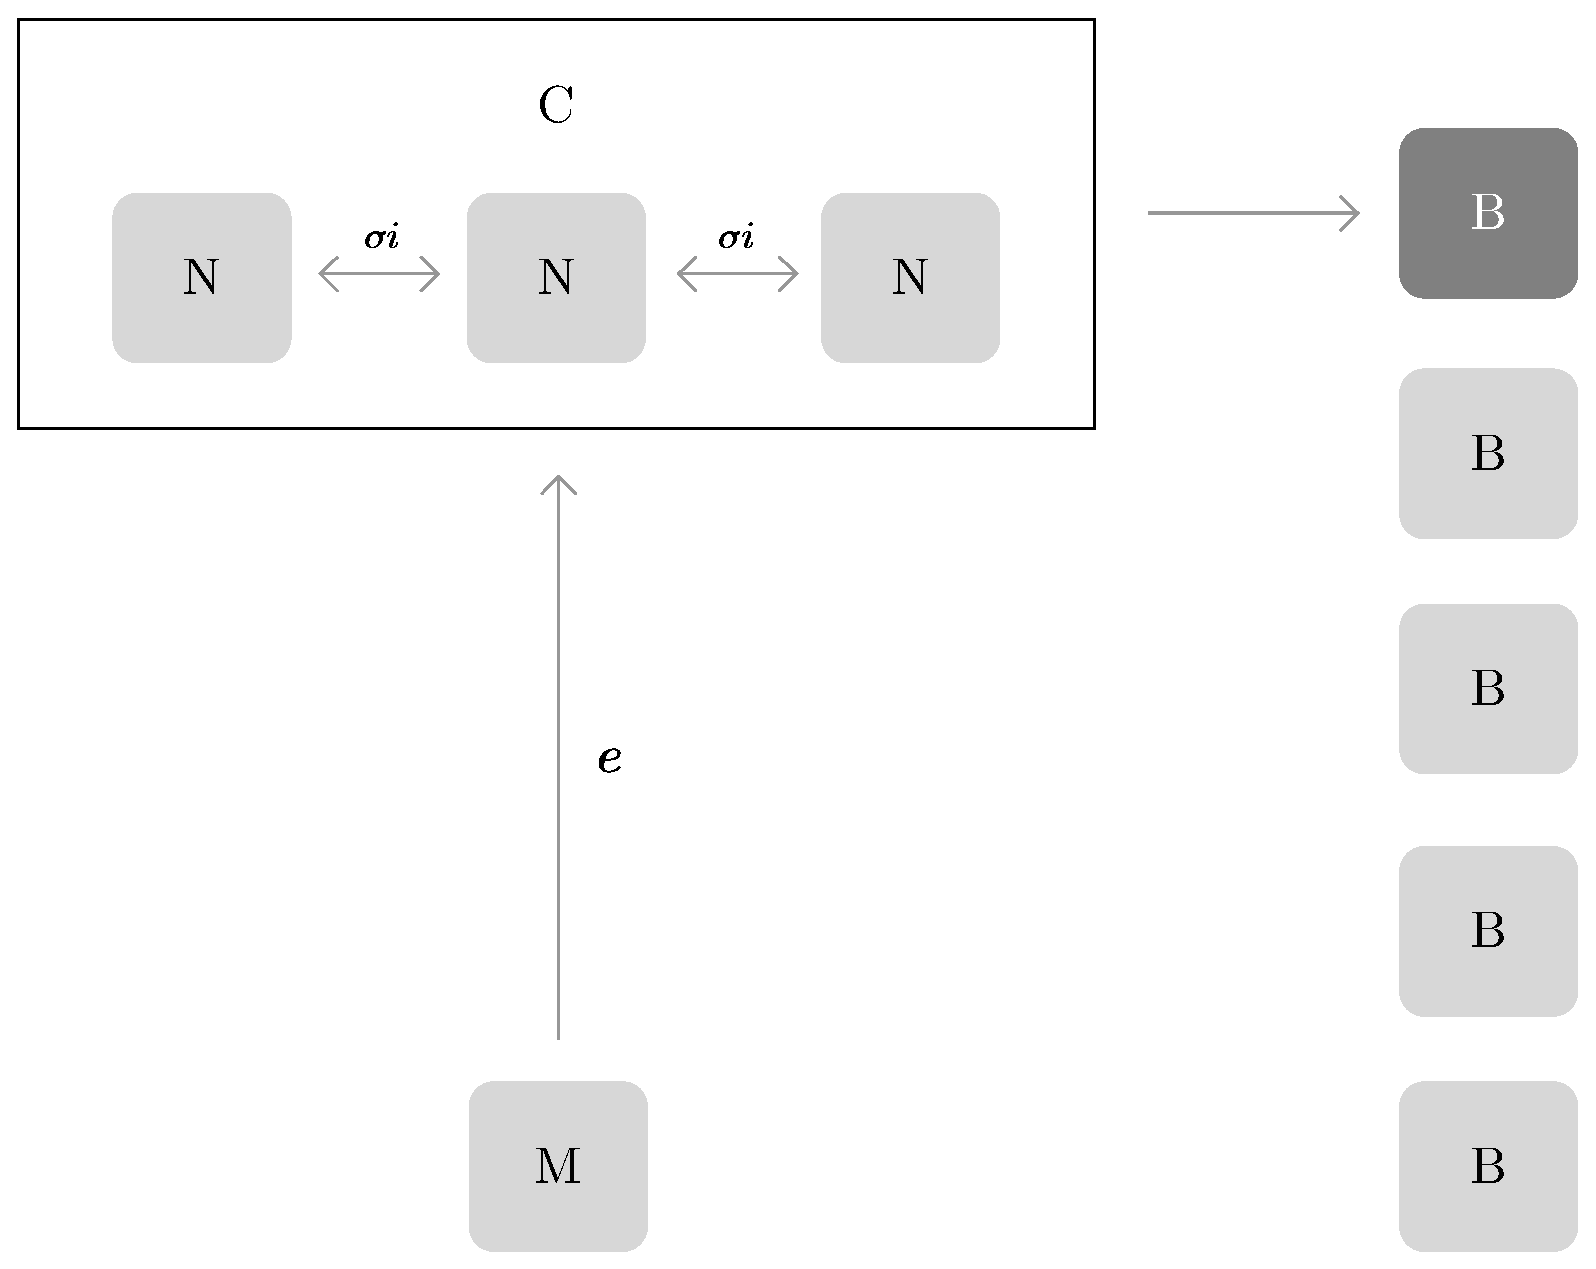
\includegraphics[width=\columnwidth]{consensus_group.eps}
          \caption{\emph{The Consensus Group and Mining}}\label{fig:consensus-group}
     \end{center}
\end{figure}

\subsubsection{Conclusion}

We have presented the Helium Consensus Protocol which combines a modern, asynchronous and highly efficient byzantine fault tolerant consensus protocol with a novel mechanism for substituting permissioned identity with a useful and reusable \emph{Proof-of-Coverage}. The resultant protocol satisfies the design requirements of being permissionless, decentralized, byzantine fault tolerant, based on useful work, and with a very high-rate censor proof transaction mechanism.

We refer the interested reader to \cite{honeybadger} for a detailed breakdown and analysis of the HoneyBadgerBFT protocol.

\section{Future Work}

This paper presents a well thought-out design for building the Helium network. However, we consider this to be just the beginning of the engineering, research and design of decentralized wireless networks. We believe that this tight integration of real-world hardware with a blockchain and a native token is a novel and valuable innovation that can be applied to other kinds of networks and wireless physical layers. We believe that the future of blockchains is not about who has the most hashing power or access to the cheapest electricity, but about blockchains where the mining proof is tied to providing a valuable, verifiable service.

There are several initiatives that we either have or intend to undertake, including:

\begin{itemize}
    \item Investigate the applicability of applying these ideas to other physical layers such as WiFi, Bluetooth and Cellular
    \item Explore the potential for the delivery of 5G 60GHz+ mmWave connectivity through a similar design
    \item Research and implement more \emph{Proofs-of-Coverage} to keep the Helium network secure as it grows
    \item Game theoretical analysis of the incentive system
    \item Formally prove the scoring algorithm used in the \emph{Proof-of-Coverage}
    \item Create and release the \emph{WHIP} wireless specification
    \item Manufacture Hotspots and Device modules for availability at launch of the Helium network
    \item Investigate the deployment of a smart contract environment beyond the basic \verb|DWN| primitives
    \item Continued work and evolution of Forward Error Correction techniques
\end{itemize}

\acks

This document is the result of collaborative work by members of our team, and would not have been possible without the help, feedback, and review of our board of directors, advisors, investors and collaborators. We extend our most heartfelt thanks to all involved.

We would also like to extend our thanks to Jeremy Rubin of the MIT Digital Currency Initiative. Your earliest feedback and direction was critical to some of the design decisions and evolution of this project. We also thank the Blockchain at Berkeley team for their help and detailed review of this work.

We would also like to acknowledge many of the prior works and inventions that have allowed us to create this project, most notably Bitcoin~\cite{bitcoin} and Ethereum~\cite{ethereum}.
\newpage

\begin{thebibliography}{10}
\softraggedright

\bibitem{idc}
    Marcus Torchia, Monika Kumar.
    \emph{IDC - Worldwide Semiannual Internet of Things Spending Guide}, 2017

\bibitem{napster}
    Shawn Fanning.
    \emph{Napster - independent peer-to-peer file sharing}, 1999

\bibitem{nist}
    Mehmet Adalier.
    \emph{Efficient and Secure Elliptic Curve Cryptography Implementation of Curve P-256}

\bibitem{honeybadger}
    Andrew Miller and Yu Xia and Kyle Croman and Elaine Shi and Dawn Song.
    \emph{The Honey Badger of BFT Protocols}, 2016

\bibitem{ethereum}
    Vitalik Buterin.
    \emph{Ethereum}, 2014

\bibitem{lora}
    LoRa Alliance.
    \emph{LoRa Alliance - Wide Area Networks for IoT}, 2013

\bibitem{rpma}
    Ingenu.
    \emph{RPMA Technology}

\bibitem{ieee802_15_4}
    IEEE.
    \emph{IEEE Standard for Low-Rate Wireless Networks}, 2015

\bibitem{bitcoin}
    Satoshi Nakamoto.
    \emph{Bitcoin: A peer-to-peer electronic cash system}, 2008

\bibitem{dijkstra}
    E. W. Dijkstra.
    \emph{A note on two problems in connection with graphs}, 1959

\bibitem{hashing}
    David Karger, Eric Lehman, Tom Leighton, Matthew Levine, Daniel Lewin, Rina Panigrahy.
    \emph{Consistent Hashing and Random Trees: Distributed Caching Protocols for Relieving Hot Spots on the World Wide Web}, 1997

\bibitem{roughtime}
    Adam Langley, Google.
    \emph{Roughtime - a project that aims to provide secure time synchronisation}

\bibitem{gtp}
    Mehmud Abliz, Taieb Znati.
    \emph{A Guided Tour Puzzle for Denial of Service Prevention}, 2009

\bibitem{mobile-experts}
    Mobile Experts
    \emph{Asset Tracking IoT Devices}, 2017

\bibitem{tdoavsrssi}
    Guofang Dong, Bin Yang.
    \emph{TDOA-Based and RSSI-Based Underground Wireless Positioning Methods and Performance Analysis}

\bibitem{tdoavstoa}
    Mohamed Laaraiedh, Lei Yu, Stephane Avrillon.
    \emph{Comparison of Hybrid Localization Schemes using RSSI, TOA, and TDOA}, 2011

\bibitem{wifipositioning}
    Mohamad Yassin, Elias Rachid, Rony Nasrallah.
    \emph{Performance Comparison of Positioning Techniques in Wi-Fi Networks}, 2014

\bibitem{locationestimation}
    Muhammad Farooq-i-Azam, Muhammad Naeem Ayyaz.
    \emph{Location and Position Estimation in Wireless Sensor Networks}, 2016

\bibitem{efficient-tdoa}
    Sangdeok Kim, Jong-Wha Chong.
    \emph{An Efficient TDOA-Based Localization Algorithm without Synchronization between Base Stations}, 2015

\bibitem{recurrent-tdoa}
    Igor Olegovych Tovkach, Serhii Yakovych Zhuk.
    \emph{Recurrent Algorithm for TDOA Localization in Sensor Networks}, 2017

\bibitem{acoustic-tdoa}
    Peter W. Boettcher, Gary A. Shaw.
    \emph{A Distributed Time-Difference of Arrival Algorithm for Acoustic Bearing Estimation}

\bibitem{async-tdoa}
    Shuai He, Xiaodai Dong, Wu-Sheng Lu.
    \emph{Asynchronous Time Difference of Arrival Positioning System}, 2015

\bibitem{lorawan}
    LoRa Alliance.
    \emph{LoRaWAN - LoRa Alliance Technology}, 2014

\bibitem{iota}
    David Sønstebø, Sergey Ivancheglo, Dominik Schiener, and Serguei Popov.
    \emph{IOTA - Next Generation Blockchain}, 2015

\bibitem{filecoin}
    Protocol Labs.
    \emph{Filecoin - A decentralized storage network}, 2017

\bibitem{pos}
    Wikipedia.
    \emph{Proof-of-Stake}

\bibitem{byzantine-failures}
    K Driscoll, B Hall, M Paulitsch, P Zumsteg, H Sivencrona.
    \emph{The Real Byzantine Generals}, 2004

\bibitem{threshold-encryption}
    Joonsang Baek, Yuliang Zheng.
    \emph{Simple and Efficient Threshold Cryptosystem from the Gap Diffie-Hellman Group}, 2003

\bibitem{lightning}
    Joseph Poon, Thaddeus Dryja.
    \emph{Lightning Network - Scalable, Instant Bitcoin/Blockchain Transactions}, 2017

\bibitem{raiden}
    brainbot.
    \emph{The Raiden Network - Fast, cheap, scalable token transfers for Ethereum}, 2017

\bibitem{state-channels}
    Jeff Coleman.
    \emph{State Channels}, 2015

\end{thebibliography}

\end{document}
